\documentclass[a4paper,twoside]{article}
\usepackage{autiwa}
\usepackage{listings}
% \lstset{language=Fortran,
% basicstyle=\ttfamily\small,
% columns=flexible}
% \lstset{keywordstyle=\color{blue}\bfseries}

\title{Aide mémoire Fortran 90}
\author{Autiwa}

\newcommand{\raccourci}[1]{{\bfseries #1}}


\makeindex
\begin{document}

\tableofcontents

\clearpage

\section{Préambule}
Ceci est un tutoriel fortran 90, il a pour but de donner des astuces de programmations, des bonnes pratiques, présenter ce qui se faisait en fortran 77 et qu'il ne faut plus faire. 

Dans la suite on considèrera le format libre, c'est à dire que les lignes peuvent avoir jusqu'à 132 caractères.

\begin{important}
Ce tutoriel, même s'il n'en est pas qu'une pâle copie est largement inspiré du tutoriel de Michel Dobrijevic pour certaines parties où je ne pouvais de tout façon pas mieux expliquer qu'il ne l'avait déjà fait. C'est avec ce tutoriel que j'ai appris \textbf{fortran 90}
\end{important}


\section{Compilation}
Le compilateur traduit les instructions qui ont été tapées par le programmeur et produit, si aucune erreur n'a été faite, en langage machine. La traduction est placée dans un fichier objet dont le nom est identique à celui du fichier source, mais dont l'extension est cette fois .o sous UNIX. Ceci est schématisé sur \reffig{fig:compilation}

\begin{attention}
Dans certains cas, l'éditeur de liens est automatiquement appelé et rend le programme exécutable.
\end{attention}

\begin{figure}[htb]
\centering
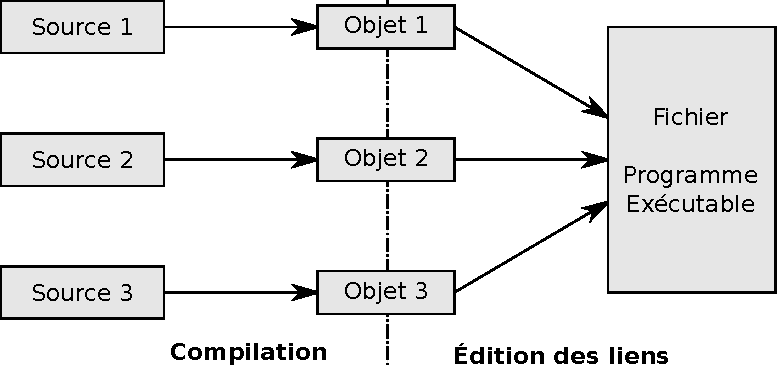
\includegraphics[width=0.65\linewidth]{figure/compilation.pdf}
\caption{La compilation de tous les fichiers source doit se faire avant l'édition des liens pour créer le fichier exécutable.}\label{fig:compilation}
\end{figure}

L'application complète comportera tous les modules liés. Tout d'abord, il conviendra de compiler séparément sans édition des liens chaque module. À l'issue de cette opération, on obtiendra des modules objets, c'est à dire en langage machine, mais sans adresse d'implantation en mémoire. On les reliera tout en fixant les adresses à l'aide de l'éditeur de liens. Le fichier obtenu sera le programme exécutable. Ceci est schématisé sur \reffig{fig:compilation_modulaire}

\begin{figure}[htb]
\centering
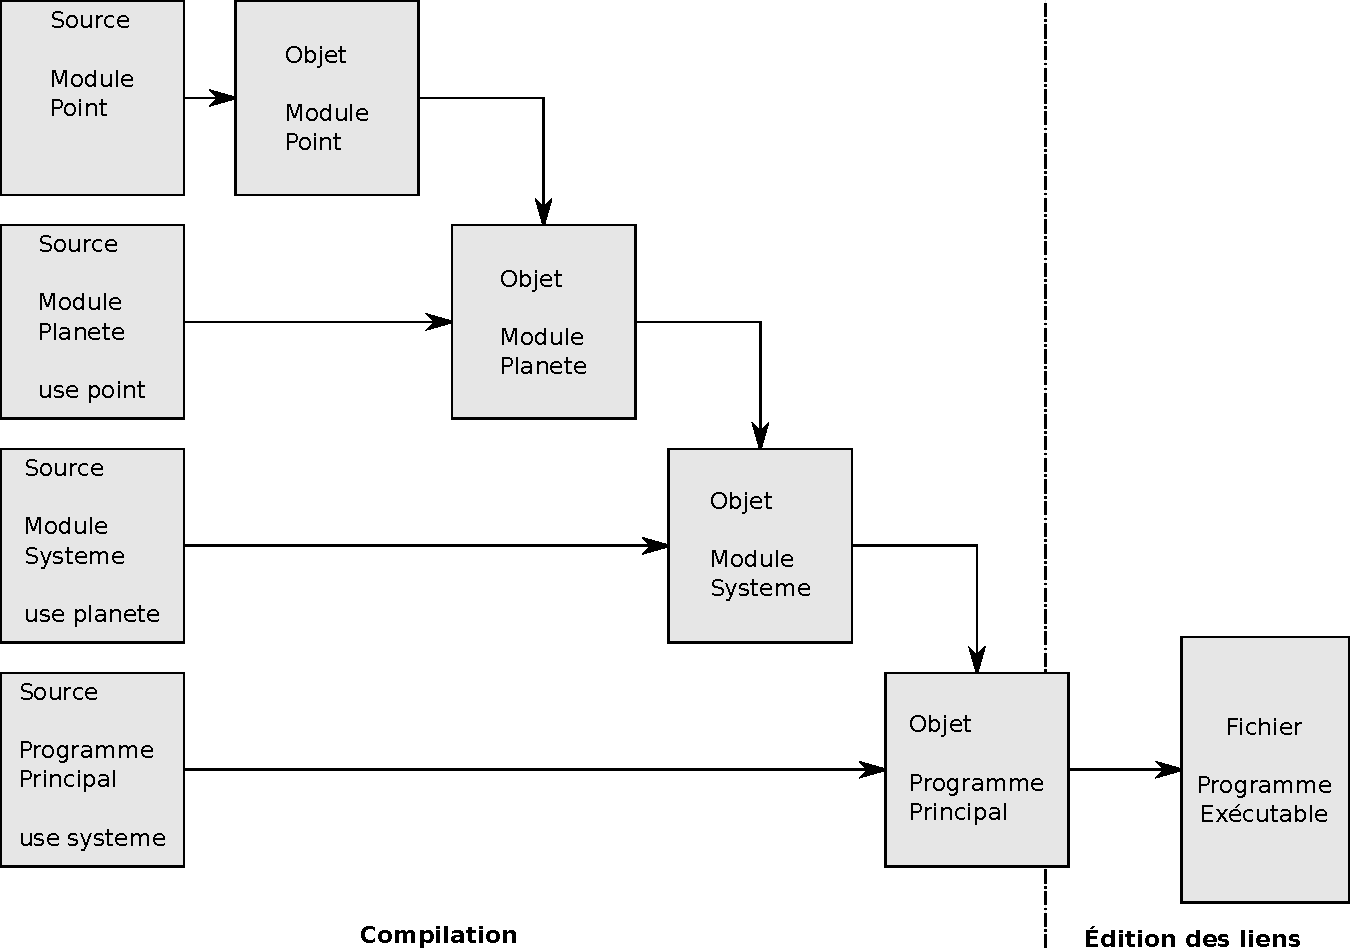
\includegraphics[width=0.65\linewidth]{figure/compilation_modulaire.pdf}
\caption{Dans le cas présent, on doit compiler le module point, puis compiler le module planète, puis compiler le module système, et enfin compiler le programme qui fait appel au module système. La compilation d'un fichier source doit se faire \emph{après} la compilation de tous les modules dont il dépend.}\label{fig:compilation_modulaire}
\end{figure}

\begin{attention}
La compilation d'un fichier source doit se faire \emph{après} la compilation de tous les modules dont il dépend.
\end{attention}


\section{Transition fortran 77/fortran 90}
\subsection{Instructions obsolètes ou dépréciées}

\begin{center}
\begin{tabular}{ll}
Obsolètes & Déprécié\\
IF arithmétique & format fixe\\
GO TO assigné & COMMON\\
RETURN multiple & DATA au milieu des inst.\\
FORMAT assigné & BLOCK DATA\\
DO sur une même instruc. & EQUIVALENCE\\
Index réel de boucle DO & GO TO calculé\\
branchement sur END IF & INCLUDE\\
PAUSE & ENTRY\\
descripteur H & DOUBLE PRECISION\\
 & Instructions Fonction\\
 & SEQUENCE\\
 & DO WHILE
\end{tabular}
\end{center}

\subsection{Comparaison f77/f90}
En fortran 77, voici les temps d'exécution : 
\begin{verbatim}
arguin.login> gfortran -o timings timings.f
arguin.login> ./timings 
 \nInteger powers tests:
 A**4 Duration=          1.3177989999999999     
 A**N (N=4) Duration=    2.4546269999999994     
 A*A*A*A Duration=       1.2278140000000004     
 \nLook-up table tests:
 Lookup table created, duration=       5.0052380000000003     
 Repeated pi/4 & sine, duration=       6.3040409999999998     
 Repeated sine, duration=       12.620081000000003     
 All lookups, duration=       1.2658079999999998     
 \nLarge array tests:
 X outer, Y inner, duration=       14.059861999999995     
 Y outer, X inner, duration=       5.0562309999999968   
\end{verbatim}

En fortran 90, en adaptant simplement le code :
\begin{verbatim}
arguin.login> gfortran -o timings timings.f90
arguin.login> ./timings 
 \nInteger powers tests:
 A**4 Duration=          1.3827890000000000     
 A**N (N=4) Duration=    2.9805470000000005     
 A**pN (pointer) Duration=    2.9005589999999994     
 A*A*A*A Duration=       1.2208150000000009     
 \nLook-up table tests:
 Lookup table created, duration=      9.99000000000194177E-004
 Repeated pi/4 & sine, duration=       1.0698379999999990     
 Repeated sine, duration=       12.619081000000000     
 All lookups, duration=       1.1228300000000004     
 \nLarge array tests:
 X outer, Y inner, duration=       12.905039000000002     
 Y outer, X inner, duration=       4.9852419999999995  
\end{verbatim}
Ce que j'ai fait : 
\begin{itemize}
\item enlever les labels dans les boucles \textbf{do}
\item rajouter un test de plus où je défini un pointeur vers l'exposant. 
\end{itemize}



\section{Les bases}
\subsection{Éléments de syntaxe}
Une ligne ne peut dépasser 132 caractères. Il est possible cependant d'étendre une instruction de plus de 132 caractères sur plusieurs lignes.

Pour continuer une ligne, en cas de ligne trop longue : 
\begin{lstlisting}[language=Fortran]
print *, 'Montant HT :', montant_ht, & 
  'TVA:',tva	,&
  'Montant TTC :', montant_ttc
\end{lstlisting}

\bigskip

Pour continuer une chaîne de caractère par contre, il faut impérativement utiliser deux caractères \og \& \fg : 
\begin{lstlisting}[language=Fortran]
print *, 'Entrez un nombre entier & 
	&compris entre 100 & 199'
\end{lstlisting}

\bigskip

Les commentaires commencent par le symbole \og ! \fg : 
\begin{lstlisting}[language=Fortran]
if (n < 100 .or. n > 199) ! Test cas d'erreur
! On lit l'exposant
read *,x 
! On lit la base
read *,y 
if (y <=0) then ! Test cas d'erreur 
  print *, 'La base doit etre un nombre > 0'
else 
  z = y**x ! On calcule la puissance
end if
\end{lstlisting}

\bigskip

\textbf{Les identificateurs.} On appelle identificateurs, les noms des variables, des fonctions, des
sous-programmes... Ils obéissent aux règles suivantes :
\begin{itemize}
\item ils sont composés de lettres (les 26 lettres de l'alphabet) et de chiffres (de 0 à 9) dont la totalité ne peut dépasser 31 caractères.
\item ils commencent obligatoirement par une lettre.
\item le symbole \og souligné\fg (\_) est un caractère utilisable par les identificateurs (à ne pas confondre avec le signe moins : \og -\fg).
\item il n'y a pas de distinction entre les minuscules et les majuscules.
\end{itemize}

\subsection{Déclaration de variables}
Le premier bloc d'instructions d'un programme source est composé de la suite de déclaration des types des différentes variables utilisées dans le programme. En fait, Fortran ne rend pas obligatoire les déclarations de type. Si une variable commence par i, j, k, l, m ou n, Fortran 90 considère par défaut que cette variable est entière. Nous déconseillons cependant fortement d'utiliser un typage implicite qui est source de nombreuses erreurs de calcul. Il est donc conseillé de commencer chaque programme par l'instruction \textbf{implicit none} qui rend obligatoire la déclaration du type de toutes les variables. Si une ou plusieurs variables ne sont pas déclarées, le compilateur retournera un message d'erreur.

La syntaxe de déclaration des variables est la suivante : 
\begin{lstlisting}[language=Fortran]
type [,attribut] :: liste_variables
\end{lstlisting}
\begin{itemize}
\item \texttt{type} est le nom du type de variable (integer, real, double precision, complex, logical, character)
\item \texttt{attribut} est une liste d'attributs optionnels (parameter, dimension, allocatable, intent,\dots)
\item \texttt{liste\_variables} est la liste des variables que l'on déclare comme ayant ce type.
\end{itemize}

\begin{exemple}
\begin{lstlisting}[language=Fortran]
program declaration
       
implicit none          
integer ::          i, j=5           ! type entier
real ::             var, x=2.5       ! type reel simple precision 
double precision :: plus_precis      ! type reel double precision 
logical ::          reussite         ! type logique 
character (10) ::   mot              ! type caractere
complex ::          z = (1.2, 20)    ! type complexe
   
[...]                      ! bloc d'instructions executables
      
end
\end{lstlisting}
\end{exemple}

Le type \texttt{logical} n'admet que deux valeurs \texttt{.true.} ou \texttt{.false.}

\begin{remarque}
Il est possible, voire recommande, d'écrire la déclaration des variables sur plusieurs lignes afin d'en faciliter la lisibilité et d'ajouter des commentaires.

\begin{lstlisting}[language=Fortran]
program commentaires 
 
implicit none
integer :: i, &       ! indice de boucle sur le temps
           j, &       ! nombre de niveaux  
           k          ! indice de boucle sur les niveaux 
    
[...]            ! bloc d'instructions executables
  
end
\end{lstlisting}
\end{remarque}

\subsection{Afficher et lire des informations (entrée et sortie standard)}
Pour pouvoir écrire des informations à l'écran, c'est-à-dire des commentaires ou le contenu de certaines variables, on utilise l'instruction print. L'affectation d'une variable par l'intermédiaire du clavier se fait en utilisant l'instruction read. Si on ne veut pas imposer le format d'écriture (on laisse faire l'ordinateur), on utilise le format par défaut symbolisé par une * (voir l'exemple du programme ecriture-lecture). Tous les caractères compris entre ' ' (ou entre ” ”) sont écrits à l'écran.

\begin{lstlisting}[language=Fortran]
program ecriture_lecture
implicit none
real :: var, &
	lu	! variable lue au clavier

var = 2.5

print*, 'La variable var vaut : ', var
print*, 'Entrez une valeur au clavier'
read*, lu
print*, 'La valeur entree au clavier est', lu

end
\end{lstlisting}

\subsection{Les expressions arithmétiques}
On retrouve les opérateurs arithmétiques usuels : \og + \fg, \og - \fg, \og * \fg et \og / \fg. Ces opérandes ne sont définis à priori que lorsque les deux opérandes sont de même type. Le résultat est du même type que les opérandes. 

Le compilateur convertit le type de l'un des opérandes, lorsque ces derniers sont différents, pour effectuer l'opération. Les conversions se font suivant la hiérarchie suivante : entier $\rightarrow$ réel $\rightarrow$ double précision. En présence d'un opérande entier et d'un opérande réel, l'entier est transformé en réel. 

\subsubsection{Cas de la division}
Ainsi le quotient de deux entiers et un entier : 
\begin{align}
\frac{5}{2} &= 2 & \frac{3}{5} &= 0
\end{align}

En revanche :
\begin{align}
\frac{5.0}{2.0} &= 2.5 \frac{5.0}{2} = \frac{5}{2.0} = 2.5
\end{align}

\subsubsection{L'opérateur d'élévation à la puissance}

L'opérateur d'élévation à la puissance se note "**". L'expression \texttt{a**b} correspond à la notation mathé\-ma\-tique $a^{b}$. 

Le résultat de l'expression \texttt{a**b} est entier si $a$ et $b$ sont entiers, sinon le résultat est réel.

Soit $b$ un entier positif, 
\begin{align}
a**b &= a*a*\ldots*a \text{ (\emph{b} fois)}\\
a**(-b) &= 1/(a**b)
\end{align}

Pour $b$ réel quelconque et $a$ positif,
\begin{align}
a**b &= exp(b*ln(a))
\end{align}

\subsection{Les expressions logiques}
Pour comparer deux expressions, Fortran 90 dispose de 6 opérateurs de comparaison, \og $<$\fg, \og $<=$\fg, \og $>$\fg, \og $>=$\fg, \og $==$\fg, \og $/=$\fg qui signifient respectivement, inférieur à, inférieur ou égal à, supérieur à, supérieur ou égal à, égal à, différent de. 

\begin{itemize}
\item Lorsque les deux expressions à comparer ne sont pas du même type, Fortran convertit le résultat de l'une des expressions dans le type de l'autre suivant les règles décrites précédemment.

\item Il faut éviter d'utiliser la comparaison entre expressions non 
entières : l'expression logique ($a == 0.0$) avec $a$ réel n'a pas grande 
signification ! 
\end{itemize}

Fortran dispose aussi d'opérateurs logiques permettant de 
combiner des opérateurs de compa\-rai\-son qui sont, par ordre de 
priorité décroissante : \og .not. \fg, \og .and. \fg, \og .or. \fg. Ils ont une 
priorité inférieure aux opérateurs précédents. 

Par exemple :
\begin{align}
y = (\mbox{.not.}(a<b)) &\equiv y = (a>=b) 
\end{align}

La variable $y$ est de type \texttt{logical}. Les parenthèses ne sont 
pas obligatoires mais facilitent la lecture (notez les points 
obligatoires de part et d'autre de \texttt{not},\texttt{and} et \texttt{or}).

\subsection{Les expressions constantes}\label{sec:constantes}
Lorsqu'une constante est utilisée plusieurs fois dans un programme (par exemple $\pi$), il est utile (et recommandé) de la définir une seule fois en début de programme pendant la déclaration des variables.
 
Deux syntaxes sont possibles :
\begin{lstlisting}[language=Fortran]
integer :: nb = 5
real :: PI = 3.141593
\end{lstlisting}
Dans ce cas les variable \emph{nb} et \emph{PI} peuvent être modifiées dans le programme.

\begin{lstlisting}[language=Fortran]
integer, parameter :: nb = 5
real, parameter :: PI = 3.141593
\end{lstlisting}
\emph{nb} et \emph{PI} sont alors des constantes symboliques dont les valeurs ne peuvent pas être modi\-fiées durant le programme (le compilateur affiche un message d'erreur s'il trouve dans le corps du programme l'instruction \texttt{nb = 12} par exemple).

Les déclarations de constante symbolique se font avant toute autre déclaration. On peut aussi utiliser une expression constante dans la mesure ou le compilateur peut la calculer. 

\begin{lstlisting}[language=Fortran]
implicit none
  
integer, parameter ::   nb = 5
integer, parameter ::   nb_max = 2*nb+4
integer, parameter ::   nb_min = 2*nb-4
integer, parameter ::   nb_elem = nb_max - nb_min + 1

[...]        ! bloc d'instructions executables 

end
\end{lstlisting}

\subsection{Les instructions de contrôle}
\subsubsection{L'instruction \emph{if} structuré}

La forme la plus générale du \texttt{if} structuré peut être 
schématisée comme suit :
\begin{lstlisting}[language=Fortran]
if (exp_log1) then
    bloc1     ! bloc d'instructions 
[else if (exp_log2) then 
    bloc2     ! bloc d'instructions 
]...
[else
    blocn     ! bloc d'instructions 
] 
end if
\end{lstlisting}
où \emph{exp\_log} est une expression quelconque de type \texttt{logical} (par exemple : \texttt{if (a $>$= 0) then} ), \emph{bloc} est un bloc d'instruc\-tions, \mbox{[ ]} signifie que le contenu est facultatif, \mbox{[ ]\ldots} signifie que le contenu peut apparaître plusieurs fois. Dans l'exemple ci-dessus, si l'expression \emph{exp\_log1} est vraie alors la suite d'instruc\-tions \emph{bloc1} est exécutée. 

Sinon, si l'expression \emph{exp\_log2} est vraie alors c'est la suite d'instruction \emph{bloc2} qui est exécutée (et ainsi de suite). Enfin, si toutes les expressions précédentes (\emph{exp\_log1}, \emph{exp\_log2}, \ldots) sont fausses et si l'instruction \texttt{else} est présente, la suite d'instructions \emph{blocn} est exécutée. Si l'instruc\-tion \texttt{else} est absente, il est possible qu'aucune instruction ne soit exécutée par un bloc \texttt{if}.

\begin{remarque}
Il est recommandé d'indenter (décaler les blocs d'instructions vers la droite d'un certain nombre de caractères blancs) les différents \texttt{if} afin d'assurer cette lisibilité. 
\end{remarque}



Un exemple d'utilisation du \texttt{if} structuré est donné dans l'exemple ci-après. 
\begin{lstlisting}[language=Fortran]
program nom_if

implicit none

integer :: i, j

read*, i, j

if (i < 0) then
  print*, 'i est negatif'
else if (i > 0) then
  print*, 'i est positif'
else
  if (j < 0) then
      print*, 'j est negatif'
  else if (j > 0) then
      print*, 'j est positif'
  else
      print*, 'i et j sont nuls'
  end if
end if

end
\end{lstlisting}

\subsubsection{L'instruction \emph{select case}}

La syntaxe générale est la suivante : 
\begin{lstlisting}[language=Fortran]
select case (exp_scal) 
[case (selecteur1)
    bloc1     ! bloc d'instructions 
[case (selecteur2)
    bloc2     ! bloc d'instructions
]... 
end select [nom]
\end{lstlisting}
où \emph{exp\_scal} est une expression de type \texttt{integer}, \texttt{logical} ou \texttt{character}. \emph{selecteur} est une valeur, un intervalle de valeurs ou une liste de valeurs de même type que \emph{exp\_scal}.

Cette instruction permet d'exécuter la suite d'instructions \emph{bloc1} lorsque la valeur de l'expression \emph{exp\_scal} est égale au \emph{selecteur} (ou dans l'intervalle donné par le \emph{selecteur}). Les intervalles sont de la forme suivante : \texttt{[valeur1]:valeur2} ou \texttt{valeur1:[valeur2]} (par exemple \texttt{case(1:)} signifie que l'on s'intéresse aux valeurs entières comprises entre 1 et 2147483647. Les sélecteurs peuvent faire appel à des expressions constantes. Les valeurs figurant dans les différents sélecteurs d'une même instruction \texttt{select case} ne doivent pas se recouper (cela engendre une erreur à la compilation).

\begin{lstlisting}[language=Fortran]
program case

implicit none

character(3) :: reponse

print*, 'Voulez-vous continuer le programme ?'
read*, reponse

select case (reponse)
  case ('oui')
    print*, 'OK, ca roule...'
  case ('non')
    print*, 'Au revoir !'
    stop
  case default
    print*, 'Veuillez repondre par "oui" ou par "non"'
end select

end
\end{lstlisting}

\begin{remarque}
Pour écrire de \emph{bons} programmes fortran, il faut : 
\begin{itemize}
\item Que dans chaque \texttt{case} il y ait une seule valeur du paramètre
\item \texttt{case default} est optionnel, mais il est conseillé de toujours en mettre un, comme ça on est sur que quelque chose sera exécuté.
\item \texttt{case default} est optionnel mais il vaut mieux le placer à la fin du \texttt{select case}, c'est plus logique et naturel.
\end{itemize}
\end{remarque}

\subsubsection{La boucle for}
La syntaxe générale est la suivante :
\begin{lstlisting}[language=Fortran]
do var = debut, fin, [pas] 
  bloc     ! bloc d'instructions 
end do
\end{lstlisting}

La variable de contrôle \emph{var} est de type \texttt{integer} ainsi que les expressions \emph{debut}, \emph{fin} et \emph{pas}.

Cette instruction permet de répéter le bloc d'instructions \emph{bloc} en donnant successivement à la variable \emph{var} les valeurs \emph{debut}, \emph{debut+pas}, \ldots, \emph{fin}. Si \emph{pas} est absent, il est par défaut égal à 1. La valeur de \emph{pas} peut être négative. Il faut alors que \emph{debut} soit plus grand que \emph{fin} sinon aucune instruction de \emph{bloc} ne sera effectuée. 

\begin{attention}
Il n'est pas possible de modifier, dans le bloc d'instructions de la boucle, la valeur de \emph{var} (le compilateur envoie un message d'erreur) et les modifications éventuelles lors de l'exécution de la boucle de \emph{debut}, \emph{fin} et \emph{pas} ne sont pas prises en compte. 

Il est imprudent de chercher à exploiter la valeur de \emph{var} après l'exécution de la boucle \texttt{do}. En effet, celle-ci ne prend pas nécessairement la valeur \emph{fin} comme on pourrait le penser a priori.
\end{attention}


\subsubsection{La boucle tant que}

La syntaxe générale est la suivante :
\begin{lstlisting}[language=Fortran]
do while (exp_log) 
    bloc     ! bloc d'instructions 
end do
\end{lstlisting}

Cette instruction permet de répéter le bloc d'instructions \emph{bloc} tant que l'expression logique \emph{exp\_log} est vraie. Si \emph{exp\_log} est fausse dès le début, le bloc n'est pas exécuté. Sinon, le bloc d'instructions doit modifier \emph{exp\_log} pour que la boucle puisse s'arrêter.

\subsubsection{Les instructions \emph{exit} et \emph{cycle}}

L'instruction \texttt{exit} permet de sortir d'une boucle de façon anticipée. Dans l'exemple suivant, les blocs \emph{bloc1} et \emph{bloc2} sont exécutés pour \emph{var} allant de \emph{debut} à \emph{fin} tant que l'expression logique \emph{exp\_log} est fausse. 

La boucle est interrompue si $var=fin$ ou si \emph{exp\_log} est vraie. Dans le premier cas on passe au \emph{bloc3}. Dans le second cas, \emph{bloc1} est exécuté mais pas \emph{bloc2}. Ensuite, on continue la boucle \texttt{do while} tant que \texttt{.not.fini} est vrai.

Comme on le voit sur cet exemple, lorsqu'une instruction \texttt{exit} appara\^{i}t dans une boucle qui est imbriquée dans une autre boucle, elle met fin à la boucle la plus interne.
\begin{lstlisting}[language=Fortran]
do while (.not.fini)
    do var = debut, fin 
        bloc1     ! bloc d'instructions 
        if (exp_log) exit
        bloc2     ! bloc d'instructions
    end do
    bloc3       ! bloc d'instructions
end do
\end{lstlisting}
Lorsque \emph{exp\_log} est vraie, on sort de la boucle \texttt{do var}


Dans l'exemple suivant, l'instruction \texttt{exit} s'applique à la boucle \texttt{do while} grâce à l'utilisation de l'identificateur \emph{boucle\_principale}. Ainsi, si \emph{exp\_log} est vraie, ni \emph{bloc2}, ni \emph{bloc3} ne sont exécutés et on sort de la boucle \texttt{do while}.
\begin{lstlisting}[language=Fortran]
do while (.not.fini)
         do var = debut, fin 
           bloc1     ! bloc d'instructions 
           if (exp_log) exit
           bloc2     ! bloc d'instructions
         end do
         bloc3       ! bloc d'instructions
end do
\end{lstlisting}
Lorsque \emph{exp\_log} est vraie, on sort de la boucle principale \texttt{do while}

L'instruction \texttt{cycle} permet de modifier le déroulement normal d'une boucle. Dans l'exemple suivant, \emph{bloc1} et \emph{bloc2} sont exécutés pour \emph{var} allant de \emph{debut} à \emph{fin} par pas de 1. 

Si l'expression logique \emph{exp\_log} est vraie, on passe à la valeur suivante de \emph{var} sans exécuter le \emph{bloc2}. Si \emph{exp\_log} est toujours vraie, seul \emph{bloc1} est exécuté.
\begin{lstlisting}[language=Fortran]
do var = debut, fin 
  bloc1      ! bloc d'instructions 
  if (exp_log) cycle
  bloc2       ! bloc d'instructions
end do
\end{lstlisting}

\section{Les tableaux}
\subsection{Déclaration des tableaux}
Un tableau est un ensemble ordonné d'éléments de même type. Chaque élément du tableau est repéré par un indice qui précise sa position au sein du tableau. Cet indice est entier. La déclaration des tableaux s'effectue comme suit :
\begin{lstlisting}[language=Fortran]
implicit none 
  
integer, parameter ::   min = -5       
integer, parameter ::   max = 12        
integer, parameter ::   nb = 10       
integer, parameter ::   nb1 = 5, nb2 = 3       
real, dimension (nb) ::           vect_1    ! tableau de rang 1 
integer, dimension (min:max) ::   vect_2    ! tableau de rang 1
real, dimension (50) ::            vect_3   ! tableau de rang 1
integer, dimension (nb1, nb2) ::  t         ! tableau de rang 2    
real, dimension (min:max, nb2) :: tab       ! tableau de rang 2 

[...]        ! bloc d'instructions executables
 
end
\end{lstlisting}

\begin{remarque}
Quand les bornes ne sont pas spécifiées, la borne inférieure est égale à 1. Dans l'un des exemples précédents, seul \emph{nb} est donné et les indices de \emph{vect\_1} vont de 1 à \emph{nb}. 

On peut aussi écrire : \texttt{real :: vect\_1(nb)}.
\end{remarque}

\begin{itemize}
\item  le nombre de dimensions est le \textbf{rang} du tableau (\emph{vect\_1} est de rang 1 et \emph{tab} est de rang 2). Le nombre maximum de dimensions est égal à 7.

\item  le nombre de valeurs possibles pour l'indice d'une dimension donnée est l'\textbf{étendue} du tableau suivant cette dimension (\emph{vect\_2} est d'étendue 18). L'indice est compris entre la \textbf{borne inférieure} (\emph{min} dans le cas de \emph{vect\_2}) et la \textbf{borne supérieure} (\emph{max} dans le cas de \emph{vect\_2}).

\item  le nombre d'éléments du tableau est la \textbf{taille} du tableau ; c'est donc le produit des étendues de chaque dimension (\emph{tab} est de taille 54).

\item  la liste des étendues est le \textbf{profil} du tableau (\emph{tab} est de profil (18, 3)).
\end{itemize}

\subsection{Les opérations relatives aux tableaux}

\subsubsection{Affectation collective}

Soit le tableau \emph{mat} de rang 3, si on désire affecter la valeur 1 à tous les éléments du tableau \emph{mat} on effectue, dans les principaux langages de programmation (\emph{Pascal}, \emph{C}, \emph{Fortran}), la suite d'instructions du programme suivant. En Fortran 90, il est possible d'obtenir le même résultat en écrivant l'instruction : \textbf{mat = 1}


\begin{lstlisting}[language=Fortran]
implicit none 
  
integer ::   i, j, k       
integer, dimension (5, -3:2, 10) ::   mat       ! tableau de rang 3 

do i = 1, 5 
  do j = -3, 2 
    do k = 1, 10 
      mat(i, j, k) = 1 
    end do 
  end do 
end do 

! est equivalent a 
mat = 1

! ou mieux
mat(:,:,:) = 1

end
\end{lstlisting}

\begin{remarque}
Par soucis de lisibilité, il est souhaitable d'expliciter les opérations sur tableaux en utilisant 
\begin{lstlisting}[language=Fortran]
mat(:,:,:) = 1
\end{lstlisting}
au lieu de 
\begin{lstlisting}[language=Fortran]
mat = 1
\end{lstlisting}
afin de pouvoir distinguer les opérations sur tableaux des opérations sur variables simples. Ça permet d'ailleurs de voir directement le nombre de dimensions du tableau.

\end{remarque}



\subsubsection{Les expressions tableaux}

On peut affecter une expression à chaque élément d'un tableau. Par exemple, les deux blocs d'instructions du programme suivant sont équivalents.

\begin{lstlisting}[language=Fortran]
implicit none 
  
integer :: i
integer, parameter ::         dim = 12

! tableaux de rang 1
integer, dimension (dim) ::   a,b
integer, dimension (dim) ::   som, prod, racine

! tableaux de type logique
logical, dimension (dim) ::   compare

do i = 1, dim 
  som(i) = a(i) + b(i) 
  prod(i) = a(i)*b(i)
  prod(i) = 2*prod(i) + 1 
  racine(i) = sqrt(real(a(i))) 
  if (som(i) < prod(i)) then 
    compare(i) = .true. 
  else 
    compare(i) = .false. 
  endif 
end do 

! En Fortran 90, les instructions precedentes
! se simplifient de la maniere suivante : 
    
! equivalent a : som = a + b
som(:) = a(:) + b(:)
prod(:) = a(:)*b(:)
prod(:) = 2*prod(:) + 1 

! Attention les elements de a sont entiers 
racine(:) = sqrt( real(a(:)) )
compare(:) = (som(:) < prod(:)) 

end
\end{lstlisting}

\subsubsection{Initialisation des tableaux à une dimension}\label{sec:initialisation_tableau}

L'initialisation d'un tableau de rang 1 à $n$ éléments est possible en utilisant une liste de $n$ éléments définie par \emph{elem\_1,\ldots,elem\_n}. Le tableau correspondant s'écrit \texttt{(/elem\_1,\ldots,elem\_n/)}. 

Un tableau à plusieurs dimensions ne peut pas être initialisé directement. Il faut définir un tableau à une dimension et utiliser une fonction particulière qui n'est pas présentée dans ce cours : la fonction \texttt{reshape}.
 
\begin{lstlisting}[language=Fortran]
program initialisation

implicit none

integer ::                  i
integer, parameter ::       n = 5
integer, dimension(n) ::    tab1, tab2, t         ! tableaux de rang 1
integer, dimension(n) ::    tab3 = (/1,2,3,4,0/)
real, dimension(0:9) ::     angle

tab1(1) = 3 ; tab1(2) = 5 ; tab1(3) = -2 ; tab1(4) = 4 ; tab1(5) = 202

tab2 = (/ 3, 5, -2, 4, 202/)

! les affectations suivantes sont equivalentes
do i = 0, 90, 10
  angle(i/10) = i*0.5
end do

angle = (/(i*0.5, i=0, 90, 10)/)                ! boucle implicite

end
\end{lstlisting}

\subsubsection{Les sections de tableau}

\emph{Fortran 90} introduit une notion nouvelle par rapport aux langages tels 
que \emph{C} ou \emph{Pascal} qui est la section de tableau. 
L'écriture générale d'une section de tableau est la suivante :
\begin{lstlisting}[language=Fortran]
tab(borne_inf : borne_sup : pas [,...])
\end{lstlisting}


\begin{itemize}
\item \emph{tab} est le nom d'un tableau,
\item \emph{borne\_inf} est la borne inférieure de la section de tableau (c'est la borne inférieure de \emph{tab} si elle est omise), 
\item \emph{borne\_sup} est la borne supérieure de la section de tableau (c'est la borne supérieure de \emph{tab} si elle est omise),
\item \emph{pas} est le pas d'incrémentation (1 par défaut ; si le pas est négatif, la variation d'indice est rétrograde de \emph{borne\_sup} à \emph{borne\_inf}.
\end{itemize}

\begin{figure}[htb]
\centering
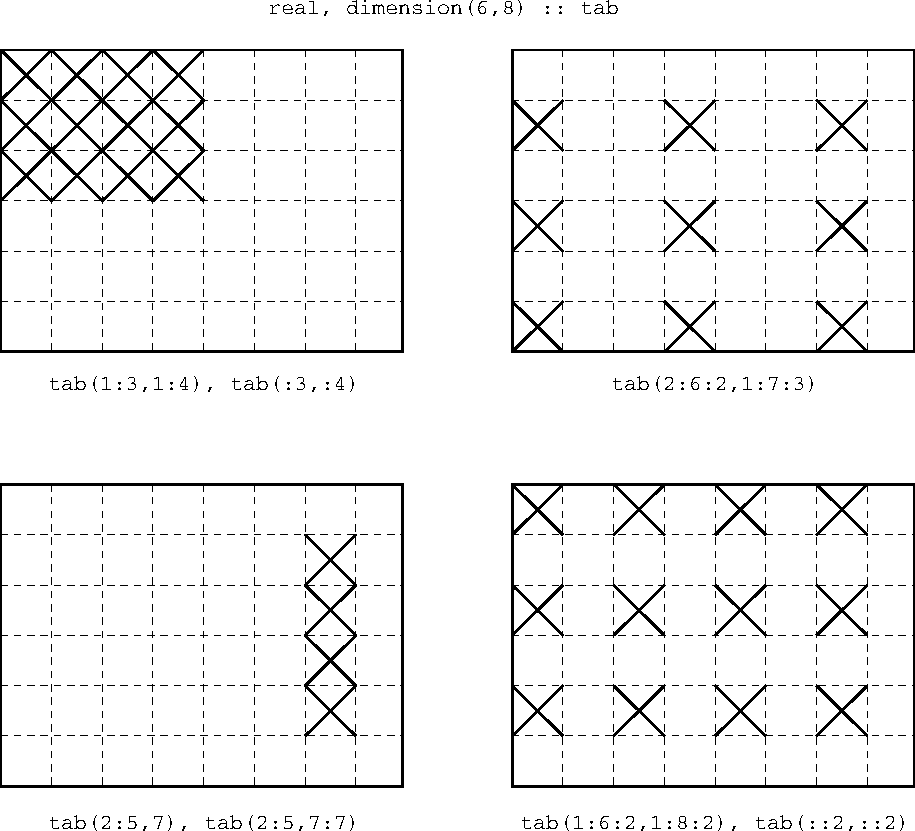
\includegraphics[width=0.65\linewidth]{figure/sections_de_tableaux.pdf}
\caption{Représentation de différentes sections de tableaux afin de montrer les possibilités de sélections.}
\end{figure}

Dans le programme suivant,
\begin{lstlisting}[language=Fortran]
integer, dimension (n) ::   w
integer, dimension (p) ::   v

v(:) = (/(i,i=1,p)/)       ! boucle implicite

! EXEMPLE 1

w(2:4) = v(7:9)
\end{lstlisting}
les valeurs  \emph{v(7)}, \emph{v(8)}, \emph{v(9)} du tableau \emph{v} sont affectées respectivement aux éléments \emph{w(2)}, \emph{w(3)} et \emph{w(4)} du tableau \emph{w}. Ainsi, la notation \texttt{w(i:j)} signifie que l'on s'intéresse aux éléments \emph{w(i), w(i+1), \ldots, w(j)} ($j>i$). 

\begin{remarque}
Si on écrit \texttt{w(3:1) = 1}, aucune affectation ne sera effectuée.
\end{remarque}

Dans le second exemple, on remarque qu'il y a un recoupement, c'est à dire que le même terme apparait à gauche et à droite du signe égal puisqu'on a les deux affectations \og simultanées\fg :
\begin{align*}
v(2) &= (v(1)+v(3))/2\\
v(3) &= (v(2)+v(4))/2
\end{align*}
Que vaut $v(2)$ dans la seconde affectation ?! 

\begin{important}
La règle adoptée par \emph{Fortran 90} est la suivante : la valeur d'une expression de type tableau est entièrement évaluée avant d'être affectée. 
\end{important}

\begin{lstlisting}[language=Fortran]
integer, dimension (n) ::   w
integer, dimension (p) ::   v, v1

v(2:9) = (v(1:8) + v(3:10))/2

! est equivalent a
do i = 1, p
  v1(i) = v(i)
end do
do i = 2, 9
  v(i) = (v1(i-1) + v1(i+1))/2
end do
\end{lstlisting}

Dans cet exemple, si on n'utilise pas les sections de tableau, on remarque qu'il est nécessaire d'utiliser un tableau tampon \emph{v1} pour effectuer les calculs intermédiaires. 

\subsubsection{Les fonctions portant sur des tableaux}

Il existe en \emph{Fortran 90} des fonctions spécifiques aux tableaux. Les plus usuelles sont \texttt{sum} qui fournit la somme des éléments d'un tableau, \texttt{maxval} qui donne la valeur maximale d'un tableau, \texttt{minval} qui donne la valeur minimale et \texttt{product} qui donne le produits des éléments. Les fonctions \texttt{dot\_product} et \texttt{matmul} permettent d'obtenir respectivement le produit scalaire et le produit matriciel de deux tableaux.

\begin{exemple}
Soit $A$ un tableau à $m$ ligne(s) et $n$ colonne(s). On cherche la valeur maximale de l'ensemble formé par les éléments se trouvant à la ligne $j$ pour les colonnes allant de $i$ à $n$. Il suffira pour cela d'écrire l'instruction suivante :
\begin{lstlisting}[language=Fortran]
maxval(A(j,i:n))
\end{lstlisting}

\bigskip

Soit $A$ une matrice de rang 2 à $n$ colonnes. L'instruction 
\begin{lstlisting}[language=Fortran]
sum(A, dim=1)
\end{lstlisting}
permet d'obtenir un tableau de rang 1 et d'étendue $n$ dont chaque élément $i$ est le résultat de la somme des éléments de la colonne $i$ de $A$.
\end{exemple}


\subsection{L'instruction \emph{where}}

Cette instruction permet de traiter les éléments d'un tableau vérifiant une certaine condition. La syntaxe est la suivante :

\begin{lstlisting}[language=Fortran]
where (inst_log_tab)
  bloc1 
[elsewhere 
  bloc2 
] 
end where
\end{lstlisting}
\emph{inst\_log\_tab} est une instruction logique portant sur les éléments d'un tableau. Lorsque cette condition est vérifiée, le bloc d'instructions \emph{bloc1} est exécuté, sinon le bloc d'instructions \emph{bloc2} est exécuté. 

Lorsque \emph{bloc1} ne contient qu'une seule instruction et que \emph{bloc2} est absent, on peut utiliser une forme simplifiée identique au \texttt{if} logique. 

Ainsi, dans l'exemple suivant, tous les éléments négatifs du tableau $A$ sont mis à zéro : 
\begin{lstlisting}[language=Fortran]
where (A < 0) A = 0.0
\end{lstlisting}

\subsection{Les tableaux dynamiques}

Quand on ne connait pas à l'avance la taille des tableaux que l'on souhaite utiliser, on peut "surdimensionner" le tableaux en question au moment de la declaration mais la méthode la plus élégante consiste à utiliser les tableaux dynamiques (tableaux à allocation différée). L'allocation sera effectuée lorsque les étendues du tableau seront connues (après lecture dans un fichier, au clavier ou après des calculs).

\bigskip

La déclaration d'un tableau dynamique s'effectue en précisant le 
rang du tableau et en utilisant l'attribut \texttt{allocatable} 
(allouable). 
\begin{lstlisting}[language=Fortran]
! declaration d'un tableau dynamique d'entiers de rang 2 
real, dimension(:,:), allocatable :: matrice
\end{lstlisting}

\bigskip

L'allocation d'un emplacement se fait en utilisant l'instruction \texttt{allocate} en précisant chaque étendue :
\begin{lstlisting}[language=Fortran]
! declaration d'un tableau dynamique d'entiers de rang 2 
real, dimension(:,:), allocatable :: matrice
integer :: n, m, verif

[...]                         ! bloc d'instructions executables

! lecture au clavier des etendues
read*, n                      ! suivant la premiere dimension
read*, m                      ! suivant la seconde dimension

allocate(matrice(n,m))
\end{lstlisting}

\begin{remarque}
Pour vérifier que l'allocation (ou la désallocation) s'est bien effectuée, on peut utiliser l'option \texttt{stat}. 
\begin{lstlisting}[language=Fortran]
allocate(matrice(n,m), stat=verif)
\end{lstlisting}
\emph{verif} est une variable entière. Si \texttt{verif = 0}, l'allocation s'est bien effectuée, sinon une erreur s'est produite. 
\end{remarque}

Lorsqu'un tableau dynamique devient inutile, il est recommandé de libérer la place allouée à ce tableau. Pour cela, on utilise l'instruction \texttt{deallocate} (désallouer).
\begin{lstlisting}[language=Fortran]
deallocate(matrice)           ! liberation
\end{lstlisting}

\bigskip

Il est possible de transmettre un tableau dynamique en argument d'une procédure sous certaines conditions : 
\begin{itemize}
\item Le tableau dynamique devra être alloué et libéré dans le programme principal. 
\item Le programme principal doit contenir l'interface de la procédure. Cette condition n'est pas obligatoire si on utilise un module! (voir par exemple le programme \emph{tableau\_dynamique}).
\end{itemize}

\begin{lstlisting}[language=Fortran]
program tableau_dynamique
 
implicit none 
! declaration d'un tableau dynamique d'entiers de rang 2 
integer, dimension (:,:), allocatable ::   matrice

integer ::   nb_lig, nb_col, i

read*, nb_lig             ! lecture au clavier du nombre de lignes
read*, nb_col             ! lecture au clavier du nombre de colonnes

! allocation d'un emplacement de profil nb_lig, nb_col
allocate (matrice(nb_lig, nb_col))    

! affectations des elements de la matrice 
do i = 1, nb_col
  matrice(:,i) = i
end do
call affiche(matrice)

! liberation de l'emplacement correspondant au tableau matrice 
deallocate (matrice) 

contains

subroutine affiche(t)
 
implicit none 
integer, dimension(:,:), intent(in) :: t      ! dimensionnement automatique
integer :: i, j 

do i = 1, size(t,1) 
  print*, (t(i,j), j=1,size(t,2))
end do

end subroutine

end 

\end{lstlisting}
Que la subroutine soit inclue dans le programme principal ou dans un module que ce dernier appelle, ça revient au même, il n'y a plus besoin de définir explicitement l'interface. Autrement il faut le faire, et ajouter
\begin{verbatim}
interface 
  subroutine affiche(t) 
    integer, dimension(:,:), intent(in) :: t 
  end subroutine affiche 
end interface 
\end{verbatim}
à la fin des déclaration de variables dans le programme principal.

\section{Les Modules}

\begin{figure}[htb]
\centering
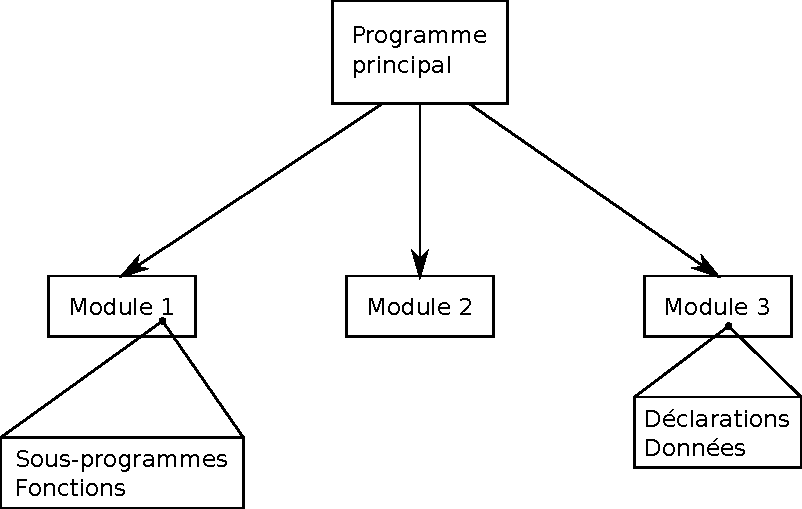
\includegraphics[width=0.65\linewidth]{figure/structure_programme.pdf}
\caption{Structure générale d'un programme Fortran 90}\label{fig:structure_programme}
\end{figure}

\reffig{fig:structure_programme} présente la structure générale d'un programme \emph{Fortran 90}. Nous allons voir qu'un programme principal peut aussi faire des appels à un ou plusieurs modules. 

\begin{definition}
Le module se présente comme une unité de programme autonome permettant de mettre des informations en commun avec d'autres unités de programmes. 
\end{definition}


Ce programme est généralement écrit dans un fichier différent du fichier contenant le programme principal. Le module est compilé indépendamment des autres unités de programme mais ne peut pas être exécuté seul. Comme le montre \reffig{fig:structure_programme}, les modules peuvent contenir des procédures (sous-programmes et fonctions), des blocs de déclarations et des données. 

Le module permet de fiabiliser les programmes en évitant la duplication des déclarations et des affectations utilisées par plusieurs unités de programme puisqu'il donne l'accès de son contenu à toutes les unités de programme qui en font l'appel.

Ils permettent : 
\begin{itemize}
\item Une écriture des sources plus simples : en particulier ils évitent d'avoir à écrire des blocs \texttt{interface} qui sont assez lourds quand ils doivent être souvent répétés
\item de remplacer avantageusement la notion de \texttt{COMMON}
\item D'accéder à toutes les ressources du \emph{Fortran 90} avec un maximum d'efficacité et de cohérence : gestion dynamique de la mémoire, pointeurs, généricité, surdéfinition des opérateurs, encapsulation\dots
\end{itemize}

\begin{attention}
Les unités \texttt{module} doivent être compilés \emph{avant} de pouvoir être utilisées. Si le fichier source est unique, elles doivent être placées en tête.
\end{attention}


\subsection{Struture générale}
Le module peut contenir un ensemble de déclarations et d'affectations et/ou une ou plusieurs procédure(s). Dans ce dernier cas, les procédures doivent être précédées par l'instruction \texttt{contains}. Un module commence par l'instruction \texttt{module} suivi du nom du module et se termine obligatoirement par \texttt{end module}.

\begin{lstlisting}[language=Fortran]
module nom_module
   
   implicit none 
   [...]         ! bloc de declarations 

   contains      ! obligatoire si suivi de procedures
   
   [...]         ! suite de procedures
 
end module nom_module
\end{lstlisting}

\subsection{Appel des modules depuis un programme principal}
L'utilisation des modules est très simple ; depuis le programme principal, l'appel du module se fait par l'instruction \texttt{use} suivi du nom du module. Il faut noter que le nom du module doit être différent de celui du programme principal. L'instruction \texttt{use} doit précéder toute autre déclaration.

\begin{lstlisting}[language=Fortran]
program utilisation_module

use nom_module 
use module_constantes

implicit none 
[...]     ! bloc de declarations

[call...
 call...] ! appels des procedures contenues dans le module nom_module
[...]     ! bloc d'instructions executables
 
end 
\end{lstlisting}

\begin{remarque}
Un module ne doit pas se référencer lui-même, même de manière indirecte. Par exemple, si le module \emph{module1} contient \texttt{use module2}, ce dernier ne doit pas contenir l'instruction \texttt{use module1}.
\end{remarque}

\subsection{Accès à tout ou partie d'un module}

Une unité de programme qui appelle un module (via l'instruction \texttt{use}) à accès à toutes les entités de ce module (variables, procédures). Il est possible cependant de contrôler l'accès à ces entités pour empêcher les conflits entre différentes unités de programme.

\bigskip

\begin{attention}
Lorsqu'une unité de programme appelle un ou plusieurs modules, il peut y avoir un conflit entre les identificateurs (noms des variables et des procédures) de l'unité de programme et des modules. Si l'on ne souhaite pas modifier les identificateurs des modules (ce qui peut être laborieux si le module est long), il est possible de renommer ces identificateurs lors de l'appel des modules à partir de l'unité de programme.
\begin{lstlisting}[language=Fortran]
use nom_module, nom_id_local => nom_id_module
\end{lstlisting}

\begin{itemize}
\item \emph{nom\_module} est le nom du module,
\item \emph{nom\_id\_local} est le nom attribué à l'identificateur 
dans l'unité de programme qui appelle le module,
\item \emph{nom\_id\_module} est le nom de l'identificateur public du 
module que l'on souhaite renommer.
\end{itemize}
\end{attention}


\begin{exemple}
\begin{lstlisting}[language=Fortran]
use module_constantes, k_bol => k
\end{lstlisting}
va permettre d'utiliser la constante $k$ du module \emph{module\_constantes} sous le nom $k_\text{bol}$ dans le programme, afin de ne pas rentrer en conflit avec une variable $k$ qui existe aussi dans le programme.
\end{exemple}


\subsubsection{Protection interne}
La première méthode pour contrôler l'accès à un module consiste à protéger certaines entités. Pour cela on utilise les instructions \texttt{private} et \texttt{public}. Par défaut, l'option d'accès au module est \emph{public}. Toutes les instructions du module se trouvant après l'instruction \texttt{private} seront d'accès privé (et donc inaccessible par le programme qui appelle le module). Il est possible aussi d'ajouter l'attribut \texttt{private} lors de la déclaration d'une variable pour protéger son accès.

\begin{lstlisting}[language=Fortran]
module module_atmosphere

use module_constantes, only : k, Na

real, private :: T = 300., &     ! temperature [K]
                 m = 28.0e-3, &  ! masse mol. moy. [gmol-1]
                 g = 9.81, &     ! pesanteur [ms-2]
                 Po = 1.01325e5  ! pression standard [Pa]

contains

function pression(z)

  real :: pression          ! pression a l'altitude z [Pa]
  real, intent(in) :: z     ! altitude [km]
  real :: h                 ! hauteur d'echelle [km]

  h = (k*T*Na)/(m*g)/1.0e3
  pression = Po*exp(-z/h)

end function pression

end module module_atmosphere
\end{lstlisting}

Et on accède au module de la façon suivante : 
\begin{lstlisting}[language=Fortran]
program acces

use module_atmosphere

implicit none

real :: p, &    ! pression [Pa]
        z       ! altitude [km]

z = 10
p = pression(z)

print*, p, g, h

end
\end{lstlisting}

Les variables \emph{T}, \emph{m}, \emph{g} et \emph{Po} ne sont pas accessibles par le programme \emph{acces} malgré l'appel du module \emph{module\_atmosphere}. Elles ont, en effet, l'attribut \texttt{private} dans \emph{module\_atmosphere}. La variable \emph{h} de la fonction \emph{pression} n'est pas en conflit avec la variable \emph{h} de \emph{module\_constantes} grâce à la restriction d'accès via l'instruction \texttt{only}.

\subsubsection{Protection externe}
La seconde méthode de contrôle d'accès entre le module et l'unité de programme qui l'appelle consiste à restreindre l'accès à certaines entités depuis l'unité de programme. Cette restriction s'effectue en utilisant l'attribut \texttt{only} lors de l'appel du module (voir le module \emph{module\_atmosphere}).
\begin{lstlisting}[language=Fortran]
use nom_module, only : liste_entites
\end{lstlisting}
où \emph{liste\_entites} est la liste des variables et procédures auxquelles on autorise l'accès lors de cet appel.



\subsection{Partage de données et variables}
Les modules peuvent être utilisés pour déclarer des variables susceptibles d'être communes à de nombreux programmes. Par exemple, un physicien est amené à utiliser, dans l'ensemble de ses programmes, les différentes constantes de la Physique. Plutôt que de déclarer ces constantes dans chaque programme, il suffit d'utiliser un module approprié dans lequel elles seront affectées une fois pour toute.

\begin{footnotesize}
\begin{lstlisting}[language=Fortran]
module module_constantes

implicit none

! Constantes de la physique en unite S.I.

real, parameter :: c = 2.99792458e8 ,  &        ! vitesse de la lumiere [ms-1]
                   G = 6.6720e-11,     &        ! constante de la gravitation [Nm2kg-2]
                   h = 6.626176e-34,   &        ! constante de planck [JHz-1]
                   k = 1.380662e-23,   &        ! constante de Boltzmann [JK-1]
                   Na = 6.022045e23,   &        ! constante d'Avogadro [mol-1]
                   Rg = 8.3145                  ! constante des gaz parfaits [Jmol-1K-1]
 
end module module_constantes
\end{lstlisting}
\end{footnotesize}

\section{Les Procédures (fonction et subroutine)}
Il existe deux types de procédures~: les sous-programmes et les fonctions (respectivement \texttt{subroutine} et \texttt{function} en anglais). Nous étudierons les fonctions plus loin dans le chapitre. Parmi les procédures, on distingue les procé\-dures externes des procédures internes.

\begin{definition}{Fonction}
Une fonction, à l'instar de son homologue en informatique, est une application qui, à partir de variable d'entrée retourne \emph{variable} de sortie qui peut être de n'importe quel type. La variable de retour est simplement une variable qui porte le même nom de la fonction et qui est retournée sans qu'on ait besoin de faire quelque chose en particulier.
\end{definition}

\begin{definition}{Subroutine}
La subroutine, contrairement à la fonction, ne distingue pas, par défaut, les variables d'entrées et de sorties, une même variable peut à la fois être une entrée et une sortie (dans la pratique, avec l'attribut \texttt{intent()} lors de la déclaration des variables on peut faire des choses un peu plus propres). 

De plus, on n'est pas limite à une variable de sortie. L'inconvénient est que, à part en regardant la déclaration ou le corps de la subroutine, on ne peut pas distinguer simplement les entrées et sorties qui sont simplement une suite de paramètres de la subroutine.
\end{definition}


\bigskip

Les sous-programmes externes (\texttt{subroutine} ou \texttt{fonction}) sont des blocs de code en dehors du programme principal, soit après son instruction \texttt{end}, soit dans un fichier séparé qu'il faudra aussi compiler. 
\begin{lstlisting}[language=Fortran]
program nom_program
 
implicit none 
[...]         ! bloc de declaration
 
[...]         ! bloc d'instructions executables
 
call nom(liste_arguments)         ! appel du sous-programme
 
[...]         ! bloc d'instructions executables
 
end  

subroutine nom(liste_arguments)

implicit none 
[...]         ! bloc de declaration (arguments et variables locales)

[...]         ! bloc d'instructions executables
 
end subroutine nom 
\end{lstlisting}


Les sous-programmes internes (\texttt{subroutine} ou \texttt{fonction}) sont des blocs de code qui vont être dans le corps du programme, à la suite de l'instruction \texttt{contains} et avant l'instruction \texttt{end}.
\begin{lstlisting}[language=Fortran]
program nom_program
 
implicit none 
[...]         ! bloc de declaration
 
[...]         ! bloc d'instructions executables 
call nom(liste_arguments)         ! appel du sous-programme 
[...]         ! bloc d'instructions executables 

contains 
subroutine nom1(liste_arguments) 
[...]         ! bloc de declaration 
[...]         ! bloc d'instructions executables 
end subroutine nom1 

subroutine nom2(liste_arguments) 
[...]         ! bloc de declaration 
[...]         ! bloc d'instructions executables 
end subroutine nom2 

end
\end{lstlisting}

Dans le cas des procédures externes, on est en présence de domaines indépendants qui ne peuvent communiquer que par le biais des arguments. 

Dans le cas des procédures internes, la procédure a accès à toutes les variables définies par son hôte. Ces variables sont dites \emph{globales} et n'ont plus besoin d'être transmises en arguments. En revanche, toutes les variables déclarées dans la procédure interne sont locales à la procédure. 

Ainsi, la déclaration de deux variables, l'une dans le programme hôte et l'autre dans la procédure interne avec le même nom provoque la création de deux variables différentes (bien qu'ayant le même nom!). Bien que pouvant paraître attrayante, cette méthode d'utilisation des procédures est à utiliser avec circonspection. En effet, l'utilisation dans le programme principal et le sous-programme interne d'un même nom pour 2 variables a priori différentes, risque de provoquer des erreurs de programmation. 


\begin{attention}
Il est important de noter que les procédures internes ne peuvent être utilisées que par l'hôte qui les contiennent. 
\end{attention}

\subsection{fonctions}
En \emph{Fortran 90}, les fonctions peuvent retourner n'importe quel type valide (tableau, type dérivé), mais une seule variable, que l'on attribue via le nom de la fonction elle même. En définissant le type de la fonction, on définit le type de la variable que l'on va retourner.

\begin{lstlisting}[language=Fortran]
function nom(liste_arguments)

implicit none 
real :: nom 
[...]         ! bloc de declaration
 
[...]         ! bloc d'instructions executables
nom = ...     ! expression arithmetique

end function nom 
\end{lstlisting}

Ainsi, la fonction \texttt{nom} retourne un réel. Ce dernier est stocké comme donnée de retour via une ligne d'attribution
\begin{lstlisting}[language=Fortran]
nom = 3e43
\end{lstlisting}
où \texttt{nom} est le nom de la fonction.

Pour appeler la fonction dans le programme principal, il suffit de faire :
\begin{lstlisting}[language=Fortran]
program nom_program 

implicit none 
real :: resultat
[...]                                  ! bloc de declaration 

[...]                                  ! bloc d'instructions executables 
resultat = 1 + 3*nom(liste_arguments)  ! exemple d'appel de la fonction nom 
[...]                                  ! bloc d'instructions executables 

end 
\end{lstlisting}

\begin{remarque}
La variable dans laquelle on stocke le résultat de la fonction doit bien évidemment avoir le même type que celui déclaré pour le nom de la fonction (et donc sa variable de retour).
\end{remarque}

\subsection{Subroutine}
En Fortran 90, une subroutine est un bloc de programme avec des entrées et des sorties. Une subroutine \texttt{transfert} s'appelle de la façon suivante : 
\begin{lstlisting}[language=Fortran]
call transfert(a,b)
\end{lstlisting}

où transfert est une subroutine qui permet d'échanger les variables $a$ et $b$ via une variable temporaire définie dans la subroutine : 
\begin{lstlisting}[language=Fortran]
subroutine transfert(a,b)

implicit none
real, intent(inout) :: a,b
real :: c

c=a
a=b
b=c
end subroutine transfert
\end{lstlisting}

Les attributs \texttt{intent(in)}, \texttt{intent(out)} ou \texttt{intent(inout)} permettent de spécifier si un argument d'une subroutine est un paramètre d'entrée, une variable de sortie ou les deux. Ce n'est pas obligatoire, mais c'est fortement conseillé de s'en servir. Sans ça, il est beaucoup plus difficile de comprendre le code, et de le sécuriser (pour savoir si on a modifié une variable alors qu'on n'aurait pas dû par exemple).

\subsection{transmission d'une procédure en argument}
Supposons que nous ayons écrit un sous programme dont l'un des arguments représente une fonction (le sous-programme utilise la fonction passée en argument). On suppose que le sous-programme est inclu dans un module. Lors de l'apparl du sous-programme depuis le programme principale, le compilateur ne pourra pas détecter que l'un des arguments est une fonction s'il n'a pas été déclaré comme tel. Pour résoudre ce problème, on utilise une interface contenant l'en-tête de la fonction ainsi que les déclarations relatives aux arguments. 
\begin{lstlisting}[language=Fortran]
program integration

! Calcul numerique d'integrales a l'aide des methodes
! composites des trapezes et de simpson

use mod_integrale

implicit none

real :: res1, res2, Pi

interface                     ! interface obligatoire
  function f1 (x)
    real, intent(in) :: x
    real :: f1
  end function
  function f2 (x)
    real, intent(in) :: x
    real :: f2
  end function
end interface

Pi = 4.0*atan(1.0)

! Appels de la subroutine sans utiliser les noms cles
! l'ordre des arguments est important
print*, ' '
call integrale (0.0, 1.0, 100, f1, res1, res2)
print*, 'Resultat de la premiere integrale : '
print*, 'Methode des trapezes : ',res1
print*, 'Methode de simpson : ',res2

! Appels de la subroutine en utilisant les noms cles
! l'ordre des arguments n'est pas important
print*, ' '
call integrale (fonction=f2, trapeze=res1, simpson=res2, &
                deb=-Pi/3.0, fin=Pi/3.0, nb_int=200)
print*, 'Resultat de la seconde integrale : '
print*, 'Methode des trapezes : ',res1
print*, 'Methode de simpson : ',res2

end program integration

function f1 (x)                  ! premiere fonction a integrer
  real, intent(in) :: x
  real :: f1
  f1 = x*x+1
end function

function f2 (x)                  ! seconde fonction a integrer
  real, intent(in) :: x
  real :: f2
  f2 = sin(x)**2.
end function
\end{lstlisting}

avec le module
\begin{lstlisting}[language=Fortran]
module mod_integrale

implicit none

contains

subroutine integrale (deb, fin, nb_int, fonction, trapeze, simpson)

  implicit none
  real, intent(in) :: deb, fin               ! bornes d'integration
  real, intent(out) :: trapeze, simpson      ! methodes d'integration
  integer, intent(in) :: nb_int              ! nb d'intervalles    
  real :: fonction

  real :: pas                                ! pas d'integration
  integer :: i

  pas = (fin - deb)/nb_int

! methode des trapezes
  trapeze = pas * ( 0.5*(fonction(deb)+fonction(fin)) + &
            sum( (/ (fonction(deb+i*pas), i = 1,nb_int-1) /) ) ) 


! methode de simpson
  simpson = pas/3.0 * ( fonction(deb) + fonction(fin) + &
            2.0*sum( (/ (fonction(deb+i*pas), i = 2, nb_int-2, 2) /) ) + &
            4.0*sum( (/ (fonction(deb+i*pas), i = 1, nb_int-1, 2) /) ) )

end subroutine integrale

end module mod_integrale
\end{lstlisting}

% %TODO page 61 les entrées et sorties standard


\section{Vers les objets : les types dérivés}\index{type dérivé}\index{structure}\index{programmation orienté objet}
On appelle type dérivé la définition d'un nouveau type de variable, sorte d'objet contenant un nombre et un type de variable arbitraire. 

\subsection{Définir un type dérivé}

Pour utiliser des variables du type dérivé \textit{nom\_type} précédemment défini, on déclare simplement :
\begin{lstlisting}[language=Fortran]
type (nom_type) [,liste_attributs] :: nom_var
\end{lstlisting}

\begin{remarque}
Pour accéder aux champs de l'objet que nous venons de définir, nous utiliserons le caractère pourcent \og \%\fg (équivalent du point pour Python par exemple). En supposant qu'un champ \textit{position} existe dans un objet \textit{planete}, on y fait appel via
\begin{lstlisting}[language=Fortran]
type (planete) :: terre

terre%position = 0.0
\end{lstlisting}
\end{remarque}

\bigskip

\begin{exemple}
Supposons qu'on veuille définir un nouveau type \textit{animal} dans lequel seraient recensés la race, l'âge, la couleur et l'état de vaccination.
\begin{lstlisting}[language=Fortran]
type animal
  character (len=20) :: race
  real :: age
  character (len=15) :: couleur
  logical, dimension(8) :: vaccination
end type animal
\end{lstlisting}

On peut ensuite manipuler globalement l'objet animal ou accéder à chacun de ses champs grâce à l'opérateur \og \%\fg.

\end{exemple}

\subsection{Initialisation lors de la déclaration}
On peut souhaiter définir une variable directement lors de la déclaration, notamment pour en faire une variable globale d'un module, donner une valeur par défaut, ou en faire un paramètre. 

Il faut alors définir la variable de la façon suivante :
\begin{verbatim}
type COULEUR
  character(len=16) :: nom
  real, dimension(3) :: compos
end type COULEUR

type(COULEUR), parameter :: coul = couleur('rouge', (/ 1.,0.,0. /))
\end{verbatim}


\section{Astuces et petits bouts de code}
\subsection{Lire un fichier de longueur inconnue}
Pour lire un fichier dont on ne connait pas le nombre de lignes : 
\begin{lstlisting}[language=Fortran]
implicit none

integer, parameter :: NMAX = 200 ! max number of messages

integer :: error
integer, dimension(NMAX) :: length
character(len=80), dimension(NMAX) :: message

open(14, file='message.in', status=old)
do
  read (14,'(i3,1x,i2,1x,a80)', iostat=error) j, length(i), message(i)
  if (error /= 0) exit
end do
close(14)
\end{lstlisting}

\begin{remarque}
La fonction \texttt{trim()} permet de supprimer les espaces en trop, pratique pour afficher ou écrire du texte proprement.
\end{remarque}

\subsection{Lire un fichier de paramètres}
Ce n'est pas \emph{la} bonne façon de faire, c'est juste ce que je fais moi. 

Je défini un caractère qui autorise des commentaires (dans mon exemple, \og !\fg). Les lignes blanches ou avec espaces sont ignorées quant à elle, vu que l'élément déclencheur est la présence du séparateur entre nom de paramètre et valeur. 

Je défini aussi un séparateur pour les paramètres (dans mon exemple \og =\fg). Chaque paramètre doit posséder un nom, sans espaces. L'ordre des paramètres n'a pas d'importance. 

\begin{remarque}
Dans le reste du programme je défini des valeurs par défaut qui seront alors écrasées lors de la lecture du fichier si le paramètre y est défini. Je défini en effet les variables en tant que variables globales du module, vu qu'elles sont constantes dans le programme (même si le fait que je ne les connaisse pas à priori m'empêche de les définir en tant que \texttt{parameter}.
\end{remarque}


\begin{lstlisting}[language=Fortran]
subroutine read_disk_properties()
! subroutine that read the 'disk.in' file to retrieve disk properties. 
! Default value exist, if a parameter is not defined

  implicit none
  
  character(len=80) :: line

  ! character that will indicate that the reste of the line is a comment
  character(len=1) :: comment_character = '!' 
  
  ! the index of the comment character on the line. 
  ! If zero, there is none on the current string
  integer :: comment_position 

  integer :: error ! to store the state of a read instruction
  
  logical :: isParameter, isDefined
  character(len=80) :: identificator, value
  !-----------------------------------------------------
  
  open(10, file='disk.in', status='old')
  
  do
    read(10, '(a80)', iostat=error), line
    if (error /= 0) exit
      
    ! We get only what is on the left of an eventual comment parameter
      comment_position = index(line, comment_character)
    
    ! If there are comments on the current line, we get rid of them
    if (comment_position.ne.0) then
      line = line(1:comment_position - 1)
    end if
    
    call get_parameter_value(line, isParameter, identificator, value)
      
    if (isParameter) then
      select case(identificator)
      case('b/h')
	read(value, *) b_over_h
      
      case('adiabatic_index')
	read(value, *) adiabatic_index

      case('temperature')
	read(value, *) temperature_0, temperature_index
	
      case default
	write(*,*) 'Warning: An unknown parameter has been found'
	write(*,*) "identificator='", trim(identificator),&
                   "' ; value(s)='", trim(value),"'"
      end select
    end if
  end do
  
  close(10)
    
end subroutine read_disk_properties
\end{lstlisting}

Dans cet exemple, je montre comment définir un paramètre ne contenant qu'une seule valeur, ou un paramètre contenant plusieurs valeurs (ici deux, mais il peut y en avoir plus). 

\begin{attention}
Notez que je ne lis que les 80 premiers caractères d'une ligne. Il ne peut donc pas y avoir de valeur définie au delà du 80\ieme caractère. Par contre, la longueur des commentaires est arbitraire, y compris sur les lignes qui contiennent des paramètres en début de ligne.
\end{attention}


Je défini ensuite la subroutine qui me permet de récupérer l'identificateur et la (ou les) valeur(s) associée(s) : 
\begin{lstlisting}[language=Fortran]
subroutine get_parameter_value(line, isParameter, id, value)
! subroutine that try to split the line in two part, 
! given a separator value (set in parameter of the subroutine)
!
! The routine return 3 values : 
!
! Return
! isParameter : is a boolean to say whether or not there is a parameter 
!  on this line. i.e if there is an occurence of the separator 
!  in the input line.
! id : a string that contain the name of the parameter
! value : a string that contains the value(s) associated with 
!  the parameter name

  implicit none
  
  ! Input
  character(len=80), intent(in) :: line
  
  ! Output
  logical, intent(out) :: isParameter
  character(len=80), intent(out) :: id, value
  
  ! Local
  ! the separator of a parameter line
  character(len=1), parameter :: sep = '=' 

  integer :: sep_position ! an integer to get the position of the separator

  !-----------------------------------------------------

  sep_position = index(line, sep)
  
  if (sep_position.ne.0) then
    isParameter = .true.
    id = line(1:sep_position-1)
    value = line(sep_position+1:)
  else
    isParameter = .false.
  end if

end subroutine get_parameter_value
\end{lstlisting}

Le fichier de paramètre est quelque chose du genre :
\begin{verbatim}
! ------------------------------------------------
! Parameter file for various properties of the disk. 
! ------------------------------------------------

adiabatic_index = 1.4
temperature = 510 1
b/h = 0.4
\end{verbatim}

\subsection{Initialisation implicite d'un tableau}
Dans la section \refsec{sec:initialisation_tableau}, une astuce est montrée pour une boucle implicite. Cette dernière est recopiée ici : 
\begin{verbatim}
angle = (/(i*0.5, i=0, 90, 10)/) ! boucle implicite
\end{verbatim}

\subsection{Remplissage d'un tableau dynamique de taille variable}
Sous ce titre flou se cache une idée simple. On veut stocker des informations sur un nombre inconnu d'évènements. Par exemple, je veux stocker la valeur des pas de temps jusqu'à un temps final. Les pas de temps étant non constants, je ne connais pas \emph{a priori} leur nombre. Ainsi, je peux faire quelque chose comme ça : 
\begin{lstlisting}[language=Fortran]
real(double_precision), dimension(:), allocatable :: time, time_temp
real(double_precision) :: time_size ! the size of the array 'time'. 
integer :: error ! to retrieve error, especially during allocations

time_size = 512 ! the size of the array. 
allocate(time(time_size), stat=error)

[...]

! If the limit of the array is reach, 
! we copy the values in a temporary array, 
! allocate with a double size, and 
! paste the old values in the new bigger array
if (k.eq.time_size) then
  allocate(time_temp(time_size), stat=error)
  time_temp(1:time_size) = time(1:time_size)
  deallocate(time, stat=error)
  time_size = time_size * 2
  allocate(time(time_size), stat=error)
  time(1:time_size/2) = time_temp(1:time_size/2)
  deallocate(time_temp, stat=error)
end if
\end{lstlisting}
où \texttt{time} est mon tableau princpal, contenant la valeur des pas de temps et \texttt{time\_temp} le tableau tampon me permettant de stocker les valeurs de \texttt{time} pendant que je l'agrandis.

Je définis \texttt{time\_size} (la taille du tableau \texttt{time}) comme étant égal à 512 au départ. Doubler la taille du tableau à chaque fois permet de limiter les réallocations qui sont coûteuses en temps. 


\section{Optimisation}
\subsection{Comparaison f77/f90}
\subsection{Profiling}
Avant d'essayer de rendre le code plus rapide, il faut en premier lieu trouver quelles parties du code le ralentissent et dans lesquelles il va être rentable de passer le temps d'optimisation.

Profiler le temps d'exécution d'un code fortran peut être fait en ajoutant l'option de compilation \texttt{-pg} : 
\begin{verbatim}
gfortran -g -pg -o myprog myprog.f90
\end{verbatim}

\begin{remarque}
Certains compilateurs, en particulier les vieux, ne vont pas autoriser les options d'optimisation si l'option \texttt{-g} est présente, et même s'ils optimisent, ça pourrait donner des résultats de profiling flous et difficiles à interpréter. 

Il vaut donc mieux éviter les options d'optimisation quand on compile pour profiler. 
\end{remarque}

Ensuite, exécutez normalement votre programme
\begin{verbatim}
./myprog
\end{verbatim}
mais il faut quand même faire attention à avoir les droits d'écriture dans le dossier d'exécution afin de pouvoir écrire le fichier de résultat du profiling, appelé \textbf{gmon.out}. 

\bigskip

Vous pouvez maintenant avoir les information de profiling en utilisant \textbf{gprof} :
\begin{verbatim}
gprof myprog gmon.out
\end{verbatim}

\begin{remarque}
Si vous voulez une analyse ligne par ligne plutôt que fonction par fonction, il vous suffit (tant que vous avez compilé le programme avec l'option \texttt{-g}), d'utiliser l'option \texttt{--line} :
\begin{verbatim}
gprof --line myprog gmon.out
\end{verbatim}
\end{remarque}

L'exécution de \textbf{gprof} va produire deux parties d'output, un \textit{flat profile} et un \textit{call graph}.
\subsubsection{flat profile}
Le flat profile ressemble à ça : 
\begin{verbatim}
Flat profile:

Each sample counts as 0.01 seconds.
  %   cumulative   self              self     total           
 time   seconds   seconds    calls  ms/call  ms/call  name    
 32.08      0.17     0.17     1488     0.11     0.14  __algo_mvs_MOD_mdt_mvs
 28.30      0.32     0.15        1   150.01   530.02  MAIN__
 16.98      0.41     0.09      477     0.19     0.34  __algo_radau_MOD_mdt_ra15
 13.21      0.48     0.07     7254     0.01     0.01  __forces_MOD_mfo_grav
  7.55      0.52     0.04     1634     0.02     0.02  __algo_mvs_MOD_mfo_mvs
  1.89      0.53     0.01     1428     0.01     0.01  __drift_MOD_drift_kepu_lag
  0.00      0.53     0.00    61641     0.00     0.00  __drift_MOD_drift_kepu_stumpff
\end{verbatim}

Ce dernier liste les sections du programme (que ce soit les fonctions ou les lignes, selon que vous utilisez ou non l'option \texttt{--line}) par ordre du temps CPU utilisé, le premier étant celui qui en utilise le plus. Chaque ligne vous donne : 
\begin{enumerate}
\item le pourcentage de CPU utilisé par cette section
\item le temps cumulé utilisé par cette section et toutes celles qui sont en dessous dans la liste
\item le nombre de seconde passés dans cette section
\item [si cette section est une fonction] : 
\begin{enumerate}
\item le nombre d'appel de cette fonction dans le programme
\item le temps moyen passé dans la fonction, par appel
\item le temps moyen passé dans la fonction, ou une des fonctions qu'elle appelle, par appel
\end{enumerate}
\item le nom de la fonction.
\end{enumerate}

\begin{remarque}
Si vous avez compilé avec l'option \texttt{-g} et l'option \texttt{--line} pour \textbf{gprof}, alors le nom de la fonction incluera aussi le nom du fichier source et le numéro de ligne. 

Le \textbf{flat profile} est suivi d'une explication de ce que signifie chaque champ.
\end{remarque}

\subsubsection{call graph}
Le \textbf{call graph} fournit les mêmes informations que le \textbf{flat profile}, mais organisation de façon à ce qu'il reflète la structure du programme. 

\begin{verbatim}
		     Call graph (explanation follows)


granularity: each sample hit covers 2 byte(s) for 1.89% of 0.53 seconds

index % time    self  children    called     name
                                   2             MAIN__ [1]
                0.15    0.38       1/1           main [2]
[1]    100.0    0.15    0.38       1+2       MAIN__ [1]
                0.17    0.05    1488/1488        __algo_mvs_MOD_mdt_mvs [3]
                0.00    0.16       1/1           mxx_sync.1545 [4]
                0.00    0.00      35/35          __algo_mvs_MOD_mco_mvs2h [13]
                0.00    0.00       1/1           __algo_mvs_MOD_mco_h2mvs [14]
                0.00    0.00    1488/1488        __dynamic_MOD_mce_cent [28]
                0.00    0.00      67/67          __mercury_outputs_MOD_mio_ce [35]
                0.00    0.00      54/54          __utilities_MOD_mio_spl [36]
                0.00    0.00      33/33          __mercury_outputs_MOD_mio_dump [37]
                0.00    0.00      32/32          __mercury_outputs_MOD_mio_out [38]
                0.00    0.00      14/15          __system_properties_MOD_mce_hill [41]
                0.00    0.00      14/14          __system_properties_MOD_mxx_ejec [42]
                0.00    0.00       6/6           __orbital_elements_MOD_mco_el2x [44]
                0.00    0.00       4/18          __system_properties_MOD_mxx_en [40]
                0.00    0.00       2/2           __mercury_outputs_MOD_mio_log [45]
                0.00    0.00       1/1           __system_properties_MOD_mce_init [47]
                                   2             MAIN__ [1]
-----------------------------------------------
                                                 <spontaneous>
[2]    100.0    0.00    0.53                 main [2]
                0.15    0.38       1/1           MAIN__ [1]
-----------------------------------------------
                0.17    0.05    1488/1488        MAIN__ [1]
[3]     40.6    0.17    0.05    1488         __algo_mvs_MOD_mdt_mvs [3]
                0.04    0.00    1490/1634        __algo_mvs_MOD_mfo_mvs [8]
                0.00    0.01   22320/25560       __drift_MOD_drift_one [10]
\end{verbatim}


\subsection{Des opérations équivalentes ne s'exécutent pas forcément avec la même rapidité}
Dans l'exemple d'un programme qui fait $X$ à la puissance $Y$, pour un entier $Y$, utilisons trois façons différentes de coder :
\begin{enumerate}
\item en utilisant la fonction power avec un $Y$ constant
\begin{lstlisting}[language=Fortran]
A=PI

call CPU_TIME(start_time)
do I=1,MAXLOOPS
    B=A**4
end do
call CPU_TIME(stop_time)
write(*,*) "A**4 Duration=       ",stop_time - start_time
\end{lstlisting}

\item en utilisant la fonction power mais avec une variable comme exposant.
\begin{lstlisting}[language=Fortran]
A=PI
N=4

call CPU_TIME(start_time)
do I=1,MAXLOOPS
    B=A**N
end do
call CPU_TIME(stop_time)
write(*,*) "A**N (N=4) Duration= ",stop_time - start_time
\end{lstlisting}

\item en multipliant $X$ par lui même $Y$ fois.
\begin{lstlisting}[language=Fortran]
A=PI

call CPU_TIME(start_time)
do I=1,MAXLOOPS
    B=A*A*A*A
end do
call CPU_TIME(stop_time)
write(*,*) "A*A*A*A Duration=    ",stop_time - start_time
\end{lstlisting}

\end{enumerate}

\begin{verbatim}
 \nInteger powers tests:
 A**4 Duration=          1.3827890000000000     
 A**N (N=4) Duration=    2.9805470000000005     
 A**pN (pointer) Duration=    2.9005589999999994     
 A*A*A*A Duration=       1.2208150000000009     
\end{verbatim}

\begin{important}
\begin{align}
A^n & \Rightarrow \underbrace{A * \cdots * A_{\text{$n$ fois}}}
\end{align}

Il vaut donc mieux élever un nombre à une puissance entière par multiplication répétée (ou multiplication répétée suivie de division par 1.0 pour les puissances d'entiers négatifs.
\end{important}

\begin{remarque}
D'autres opérations pour lesquelles il y a de multiples façon de programmer auront le même comportement. Si on a un doute sur la technique à utiliser, on peut toujours modifier les sources fournis pour créer un set de tests pour un autre type d'opération.
\end{remarque}


\subsection{Use Lookup Tables for Common Calculations}
Le code ci-dessous consiste à comparer de manière intensive une valeur calculée de $\sin\left(\frac{\pi}{4}\right)$ dans une boucle, en utilisant une valeur pré-calculée stockée dans un tableau ("lookup table").

Tout d'abord on crée les tables de données : 
\begin{verbatim}
do i=1,10
    pi_table(i)=pi/i
    sine_table(i)=sin(pi_table(i))
end do
\end{verbatim}

utilisons trois façons différentes de coder :
\begin{enumerate}
\item en calculant intégralement à chaque fois :
\begin{lstlisting}[language=Fortran]
call cpu_time(start_time)
do i=1,maxloops
    b=i*sin(pi/4.0)
end do
call cpu_time(stop_time)
write(*,*) "Repeated pi/4 & sine, Duration=    ",stop_time - start_time
\end{lstlisting}

\item en utilisant la table d'arguments :
\begin{lstlisting}[language=Fortran]
call cpu_time(start_time)
do  i=1,maxloops
    b=i*sin(pi_table(4))
end do
call cpu_time(stop_time)
write(*,*) "Repeated sine, Duration=    ",stop_time - start_time
\end{lstlisting}

\item en utilisant une table de sinus :
\begin{lstlisting}[language=Fortran]
call cpu_time(start_time)
do i=1,maxloops
    b=i*sine_table(4)
end do
call cpu_time(stop_time)
write(*,*) "All lookups, Duration=    ",stop_time - start_time
\end{lstlisting}
\end{enumerate}

On peut constater que le pré-calcul de $\pi/4$ fait peu de différence, mais éviter l'évaluation répétée de la fonction sinus (très consommatrice en temps) entraine un temps de calcul 40 fois plus court. Dans cet exemple, le temps pris par la construction de la table de valeur est beaucoup moins grand que le temps économisé par le fait de se servir de la table.

\begin{verbatim}
 Repeated pi/4 & sine, Duration=      2.99960000000000226E-002
 Repeated sine, Duration=      0.16397499999999998     
 All lookups, Duration=      1.29980000000000095E-002
\end{verbatim}

\begin{remarque}
Dans d'autres situation, la différence pourrait ne pas être aussi sensible. Cependant, il peut être parfois très intéressant de faire calculer à un autre programme une table de valeur que le programme pourra ensuite lire dans un fichier.

Quand c'est applicable, il peut être aussi intéressant de produire une table de valeur et ensuite d'interpoler la fonction entre deux valeurs tabulées pour calculer l'image par la fonction au lieu d'évaluer cette dernière à chaque fois.
\end{remarque}

\subsection{Minimiser les sauts dans l'adressage mémoire}\label{sec:indices_loops}
Cette section a pour but d'illustrer comment la manière dont est construit l'ordinateur peut influencer l'exécution de votre programme.

Tous les ordinateurs modernes ont trois types de mémoire :
\begin{itemize}
\item de la mémoire cache (quelques Mio)
\item de la RAM (environ 4 Gio)
\item de la mémoire tampon (\textit{swap}) écrite sur disque dur (quasiment autant qu'on veut)
\end{itemize}
Chacun de ces types de mémoire peut être considéré un ordre de magnitude plus lent en terme de temps d'accès par rapport au type indiqué au dessus de lui dans la liste. Idéalement on veut donc utiliser la mémoire cache au maximum, et éviter autant que possible d'avoir recours à la mémoire tampon (ou \textit{swap}). Malheureusement, vous n'avez aucun contrôle sur l'endroit où sont stockées les informations, c'est l'ordinateur qui gère les déplacements de fichiers de l'une à l'autre des types de mémoire. 

\begin{important}
À cause de ce comportement, on ne veut pas continuellement être en train de transférer des informations dans la mémoire cache parce que des informations logiques se trouvent à des emplacements physiques éloignés dans la mémoire. Il est donc important de comprendre comment est agencée la mémoire en fortran, en particulier dans les tableaux. C'est ce qu'illustre l'exemple suivant, par l'utilisant d'un grand tableau à deux dimension où on fait des opérations sur les éléments.
\end{important}

Même si \textbf{fortran} autorise l'utilisation de tableaux multi-dimensionnels, l'espace mémoire de l'ordinateur n'a qu'une seule dimension. \reffig{fig:array_indices} montre comment est représenté un simple tableau 3x3 \texttt{a(i,j)}.

\begin{figure}[htb]
\centering
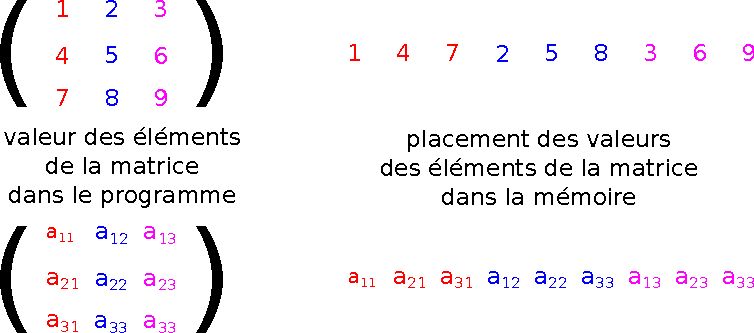
\includegraphics[width=0.65\linewidth]{figure/array_indices.pdf}
\caption{Représentation de l'agencement en mémoire des valeurs associées aux éléments d'une matrice. L'élément $a_{ij}$ (ligne $i$ et colonne $j$) est noté \texttt{a(i,j)} en \textbf{fortran 90}}\label{fig:array_indices}
\end{figure}

On constate alors que c'est l'indice $i$ qui varie le plus rapidement. 

Si on a un tableau de grande dimension, alors faire varier le deuxième indice de 1 va entrainer la mise en mémoire cache d'une autre page de données. Il est donc important de mettre les boucles dans le bon ordre sous peine de ralentir considérablement les calculs. 

\begin{remarque}
Dans la pratique, ce n'est pas si important que ça à partir du moment où on active les options d'optimisation qui vont se charger d'inverser l'ordre des boucles lors de la compilation. Mais c'est toujours bon de le savoir, ne serait-ce que pour certains cas particuliers.
\end{remarque}

On a donc les deux cas de figure suivant : 
\begin{itemize}
\item on fait varier d'abord l'indice des lignes puis pour chaque ligne on parcours toutes les colonnes
\begin{lstlisting}[language=Fortran]
call cpu_time(start_time)
do i=1,maxloops2
    do x=1,2000
      do y=1,2000
	  matrix(x,y)=x*y
      end do
    end do
end do
call cpu_time(stop_time)
write(*,*) "x outer, y inner, Duration=    ",stop_time - start_time
\end{lstlisting}

\item on fait varier d'abord l'indice des colonnes puis pour chaque colonne on parcours toutes les lignes
\begin{lstlisting}[language=Fortran]
call cpu_time(start_time)
do i=1,maxloops2
    do y=1,2000
      do x=1,2000
	  matrix(x,y)=x*y
      end do
    end do
end do
call cpu_time(stop_time)
write(*,*) "y outer, x inner, Duration=    ",stop_time - start_time
\end{lstlisting}
\end{itemize}

\begin{verbatim}
 x outer, y inner, Duration=      0.52391999999999994     
 y outer, x inner, Duration=      0.14897799999999994     
\end{verbatim}

Imbriquer les boucles dans le mauvais ordre ralenti le code par un facteur 3 environ. Il faut donc que l'indice qui varie le plus vite soit l'indice des lignes. 

\subsection{Utiliser les options d'optimisation du compilateur}
L'astuce la plus simple pour augmenter la vitesse d'exécution d'un programme est de loin d'utiliser les options d'optimisation du compilateur. 

L'option \texttt{-O2} est une sorte de meta option qui regroupe plein d'options, c'est celle qu'il faut activer en priorité. Dans mon cas, j'ai eu un gain de temps supérieur à 30\% (mais ça dépend fortement du programme).

\begin{remarque}
Avec l'option \texttt{-O2}, il n'y a plus de différence de temps entre les deux ordres de boucles pour \refsec{sec:indices_loops}.
\end{remarque}

Une autre option qui peut augmenter parfois la rapidité d'un programme est \texttt{-funroll-loops}

\section{Les fonctions intrinsèques en Fortran 90}
Voici une liste de quelques fonctions intrinsèques du \emph{Fortran 90}. 
Toutes les fonctionnalités de chaque fonction ne sont pas 
données. Pour plus de renseignements sur ces fonctions et les 
autres fonctions, consultez les ouvrages de référence (voir bibliographie).
 
\subsection{Les fonctions numériques}

\subsubsection{Les fonctions numériques élémentaires}

\begin{description}
\item[\textbf{ABS} \emph{abs(a)}]  Fournit la valeur absolue de \emph{a} ($\left|a\right|$), de type entier, réel ou complexe. Le résultat est du type de \emph{a}. Quand \emph{a} est complexe ($a=(x,y)$), le résultat est de type \emph{real} et égal à $\sqrt{x^{2}+y^{2}}$. 
\begin{exemple}
\begin{align}
\mathrm{abs}(-7.4) &= 7.4\\
\mathrm{abs}((6.0,8.0))&= 10.0
\end{align}
\end{exemple}

\item[\textbf{AIMAG} \emph{aimag(z)}] Fournit la partie imaginaire de \emph{z}, de type complexe. Le résultat est de type \emph{real}. Si $z=(x,y)$, le résultat est égal à $y$. 
\begin{exemple}
\begin{align}
\mathrm{aimag}((4.0,5.0))&= 5.0
\end{align}
\end{exemple}

\item[\textbf{AINT} \emph{aint(a)}] Fournit, dans le type \emph{real}, la troncature de \emph{a} (partie entière $E(a)$ pour $a>0$ et $-E(-a)$ pour $a<0$). 
\begin{exemple}
\begin{align}
\mathrm{aint}(3.678) &= 3.0\\
\mathrm{aint}(-1.375) &= -1.0
\end{align}
\end{exemple}

\item[\textbf{ANINT} \emph{anint(a)}] Fournit, dans le type \emph{real}, l'arrondi de \emph{a} à l'entier le plus proche. 
\begin{exemple}
\begin{align}
\mathrm{anint}(3.456) &= 3.0\\
\mathrm{anint}(-2.798) &= -3.0
\end{align}
\end{exemple}

\item[\textbf{CEILING} \emph{ceiling(a)}] Fournit l'entier (type \emph{integer} standard) immédiatement supérieur à la valeur du réel \emph{a} (voir \emph{floor}).
\begin{exemple}
\begin{align}
\mathrm{ceiling}(4.8) &= 5\\
\mathrm{ceiling}(-2.55) &= -2
\end{align}
\end{exemple}

\item[\textbf{CMPLX } \emph{cmplx(x,y)}] 
\begin{itemize}
\item Si \emph{y} est absent~: fournit le résultat de la conversion de la valeur \emph{x} (de type numérique quelconque, complexe compris) en un complexe standard, 
\item Si \emph{y} est présent~: fournit le résultat de la conversion du complexe (\emph{x},\emph{y}) (\emph{x} et \emph{y} doivent être de type entier ou réel) dans le type complexe standard. 
\end{itemize}
\begin{exemple}
\begin{align}
\mathrm{cmplx}(-3) &= (-3.0,0.0)\\
\mathrm{cmplx}(4.1,2.3) &= (4.1,2.3)
\end{align}
\end{exemple}

\item[\textbf{FLOOR} \emph{floor(a)}] Fournit l'entier (type \emph{integer} standard) immédiatement inférieur à la valeur du réel \emph{a} (voir \emph{ceiling}). 
\begin{exemple}
\begin{align}
\mathrm{floor}(4.8)  &= 4\\
\mathrm{floor}(-5.6)  &= -6
\end{align}
\end{exemple}

\item[\textbf{INT} \emph{int(a)}] Fournit le résultat de la conversion en entier standard de la valeur de \emph{a} qui peut être entière (le résultat est alors égal à \emph{a}), réelle (le résultat est aIors égal à la troncature de \emph{a}, c'est-à-dire \emph{aint(a)}) ou complexe (le résultat est alors égal à la troncature de la partie réelle de \emph{a}). 
\begin{exemple}
\begin{align}
\mathrm{int}(-4.2)  &= -4\\
\mathrm{int}(7.8)  &= 7
\end{align}
\end{exemple}

\item[\textbf{NINT} \emph{nint(a)}] Fournit l'entier standard le plus proche du réel \emph{a}. 
\begin{exemple}
\begin{align}
\mathrm{nint}(3.879)  &= 4\\
\mathrm{nint}(-2.789)  &= -3
\end{align}
\end{exemple}

\item[\textbf{REAL} \emph{real(a)}] Fournit le réel correspondant à \emph{a} qui peut être de type numérique quelconque (s'il est complexe, on obtient la partie réelle). 
\begin{exemple}
\begin{align}
\mathrm{real}(-4)  &= -4.0
\end{align}
\end{exemple}

\end{description}

\begin{remarque}
les fonctions suivantes (\emph{conjg} à \emph{sign}) fournissent un résultat ayant le même type que leur premier argument et lorsque plusieurs arguments sont prévus, ils doivent tous être du même type.
\end{remarque}

\begin{description}

\item[\textbf{CONJG} \emph{conjg(z)}] Fournit le complexe conjugué du complexe z. 
\begin{exemple}
\begin{align}
\mathrm{conjg}((2.0,3.0))  &= (2.0,-3.0)
\end{align}
\end{exemple}

\item[\textbf{DIM} \emph{dim(x, y)}] Fournit le maximum de $x-y$ et de 0, $x$ et $y$ sont entiers ou réels. 
\begin{exemple}
\begin{align}
\mathrm{dim}(6,2)  &= 4\\
\mathrm{dim}(-4.0,3.0)  &= 0.0
\end{align}
\end{exemple}

\item[\textbf{MAX} \emph{max(a1, a2, a3\dots)}] Fournit la valeur maximale des valeurs reçues en arguments (entiers ou réels). 
\begin{exemple}
\begin{align}
\mathrm{max}(2.0, -8.0, 6.0)  &= 6.0
\end{align}
\end{exemple}

\item[\textbf{MIN} \emph{min(a1, a2, a3\dots)}] Fournit la valeur minimale des valeurs reçues en arguments (entiers ou réels). 
\begin{exemple}
\begin{align}
\mathrm{min}(2.0, -8.0, 6.0)  &= -8.0
\end{align}
\end{exemple}

\item[\textbf{MOD} \emph{mod(a, p)}] Fournit la valeur de \emph{a-int(a/p)*p} ; $a$ et $p$ doivent être de même type (entiers ou réels). Si $p$ est nul, le résultat dépend de la machine (pas défini). 
\begin{exemple}
\begin{align}
\mathrm{mod}(7,3)  &= 1\\
\mathrm{mod}(9,-6)  &= 3
\end{align}
\end{exemple}

Cette fonction est souvent utilisée pour tester si un nombre est pair ou impair. 
\begin{exemple}
\begin{align}
\mathrm{mod}(4,2)  &= 0\\
\mathrm{mod}(5,2)  &= 1
\end{align}
\end{exemple}

\item[\textbf{MODULO} \emph{modulo(a, p)}] Fournit la valeur de $a$ modulo $p$, c'est-à-dire \texttt{a-floor(a/p)*p} quand $a$ et $p$ sont réels et \texttt{a-floor(a:p)*p } (\og:\fg représentant la division euclidienne quand $a$ et $p$ sont entiers). Si $p$ est nul, le résultat dépend de la machine (pas défini). 
\begin{exemple}
\begin{align}
\mathrm{modulo}(7,3)  &= 1\\
\mathrm{modulo}(9,-6)  &= -3\\
\mathrm{modulo}(156,2)  &= 0
\end{align}
\end{exemple}

\item[\textbf{SIGN} \emph{sign(a, b)}] Fournit la valeur absolue de $a$ multiplié par le signe de $b$ ($a$ et $b$ doivent être de même type). 
\begin{exemple}
\begin{align}
\mathrm{sign}(4.0,-6.0)  &= -4.0\\
\mathrm{sign}(-5.0,2.0)  &= 5.0
\end{align}
\end{exemple}

\end{description}

\subsubsection{Les fonctions mathématiques élémentaires}

\begin{remarque}
toutes ces fonctions fournissent un résultat ayant le même type que leur premier argument. L'argument \emph{x} peut être aussi un tableau. Dans ce cas, la fonction s'applique sur tous les élements du tableau.
\end{remarque}

\begin{description}
\item[\textbf{ACOS} \emph{acos(x)}] Fournit la valeur en radians, dans l'intervalle $[0,\pi]$, de arccosinus de $x$, $x$ étant un réel tel que $x \in [-1,1]$. 

\item[\textbf{ASIN} \emph{asin(x)}] Fournit la valeur en radians, dans l'intervalle $[-\frac{\pi}{2}, \frac{\pi}{2}]$, de arcsinus de $x$, $x$ étant un réel tel que $x \in [-1,1]$. 

\item[\textbf{ATAN} \emph{atan(x)}] Fournit la valeur de arctangente de $x$, $x$ étant réel, exprimé en radians, dans l'intervalle $[-\frac{\pi}{2}, \frac{\pi}{2}]$.

\item[\textbf{ATAN2} \emph{atan2(y,x)}] Fournit la valeur principale de l'argument
du nombre complexe $(x,y)$, exprimée en radians dans l'intervalle $[-\pi, \pi]$, 
$x$ et $y$ étant du même type réel. 

Les valeurs de $x$ et $y$ ne doivent pas être toutes deux nulles. 
\begin{exemple}
\begin{align}
atan2(2.679676,1.0)  &= 1.213623
\end{align}
\end{exemple}

\item[\textbf{COS} \emph{cos(x)}] Fournit le cosinus de $x$ pour $x$ réel ou complexe, exprimé en radians. 

\item[\textbf{COSH} \emph{cosh(x)}] Fournit la valeur du cosinus hyperbolique de $x$, $x$ étant un réel exprimé en radians.  

\item[\textbf{EXP} \emph{exp(x)}] Fournit la valeur de l'exponentielle de $x$ pour $x$ réel ou complexe.  

\item[\textbf{LOG} \emph{log(x)}] Fournit la valeur  du logarithme népérien de $x$, réel positif ou complexe non nul (dans ce dernier cas, le résultat possède une partie imaginaire situé dans l'intervalle $[-\pi;\pi]$).

\item[\textbf{LOG10} \emph{log10(x)}] Fournit la valeur du logarithme à base 10 du réel positif $x$. 

\item[\textbf{SIN} \emph{sin(x)}] Fournit le sinus de $x$ pour $x$ réel ou complexe et exprimé en radians.  

\item[\textbf{SINH} \emph{sinh(x)}] Fournit la valeur du sinus hyperbolique de $x$, $x$ étant réel et exprimé en radians.  

\item[\textbf{SQRT} \emph{sqrt(x)}] Fournit la valeur de la racine carrée de $x$, réel positif ou nul ou complexe (dans ce cas, le résultat possède une partie réelle non négative ; s'il s'agit de 0, la partie imaginaire du résultat n'est pas négative).

\item[\textbf{TAN} \emph{tan(x)}] Fournit la tangente de $x$ réel exprimé en radians. 

\item[\textbf{TANH} \emph{tanh(x)}] Fournit la tangente hyperbolique de $x$ pour $x$  réel et exprimé en radians.
    
\end{description}

\subsubsection{Les fonctions d'interrogation}

\begin{remarque}
Toutes ces fonctions peuvent recevoir en argument un scalaire (numérique) ou un tableau d'éléments numériques.
\end{remarque}

\begin{description}
\item[\textbf{DIGITS} \emph{digits(x)}] Fournit le nombre (entier standard) de chiffres significatifs du type de $x$ (réel ou entier). 
\begin{exemple}
si $x$ est un réel codé sur 32 bits, 
\begin{align}
\mathrm{digits}(x)  &= 24
\end{align}
\end{exemple}

\item[\textbf{EPSILON} \emph{epsilon(x)}] Fournit l'"epsilon machine" (le plus petit nombre $\epsilon$ tel que $1+\epsilon$ soit différent de 1) du type correspondant au réel $x$. Le résultat a la valeur $b^{1-p}$. 
\begin{exemple}
si $x$ est un réel codé sur 32 bits, 
\begin{align}
\mathrm{epsilon}(x)  &= 2^{-23}
\end{align}
\end{exemple}

\item[\textbf{HUGE} \emph{huge(x)}] Fournit la plus grande valeur représentable dans le type de $x$. Le résultat est du même type que $x$ qui peut être entier ou réel. Si $x$ est réel, le résultat a la valeur $(1-b^{-p})*b^{e_{max}}$.
\begin{exemple}
si $x$ est un réel codé sur 32 bits, 
\begin{align}
\mathrm{huge}(x) \rightarrow (1-2^{-24})*2^{128}
\end{align}
\end{exemple}

\item[\textbf{MAXEXPONENT} \emph{maxexponent(x)}] Fournit la plus grande valeur (entier standard) possible pour un exposant dans le type (réel) de $x$.

\item[\textbf{MINEXPONENT} \emph{minexponent(x)}] Fournit la plus petite valeur (entier standard) possible pour un exposant dans le type (réel) de $x$.

\item[\textbf{PRECISION} \emph{precision(x)}] Fournit le nombre (entier standard) minimal de chiffres significatifs dans le type (réel ou complexe) de $x$.

\item[\textbf{RANGE} \emph{range(x)}] Fournit la valeur maximale \emph{e} (entier standard) d'un exposant (en puissance de 10) dans le type de \emph{x} (entier, réel ou complexe) telle que les nombres $10^{e}$ et $10^{-e}$ soient représentables dans le type en question. 
\begin{exemple}
si $x$ est un réel codé sur 
32 bits, 
\begin{align}
\mathrm{range}(x)  &= 37
\end{align}
\end{exemple}

\item[\textbf{TINY} \emph{tiny(x)}] Fournit la plus petite valeur représentable dans le type de $x$. Le résultat est du même type (variante comprise) que $x$ qui peut être réel ou double précision. Le résultat a la valeur $b^{e_{min}-1}$. 
\begin{exemple}
si $x$ est un réel codé sur 32 bits, 
\begin{align}
\mathrm{tiny}(x)  &= 2^{-126}
\end{align}
(environ $10^{-38}$).
\end{exemple}
    
\end{description}

\subsection{les fonctions relatives aux chaînes de caractères}

\subsubsection{Les fonctions élementaires}

\begin{description}

\item[\textbf{CHAR} \emph{char(i)}] Fournit une chaîne de caractères de longueur 1 correspondant au caractère de code ASCII \emph{i} (entier). 
\begin{exemple}
\begin{align}
\mathrm{char}(71)  &= 'G'\\
\mathrm{char}(63)  &= '?'
\end{align}

\end{exemple}

\item[\textbf{ICHAR} \emph{ichar(c)}] Fournit l'entier (type \emph{integer} standard) correspondant au code ASCII du caractère \emph{c}  (chaîne de longueur 1). 
\begin{exemple}
\begin{align}
\mathrm{ichar}('Y')  &= 89\\
\mathrm{ichar}('\%')  &= 37
\end{align}

\end{exemple}

\end{description}

\subsubsection{Les fonctions de comparaison de chaînes}

\begin{description}
    
\item[\textbf{LGE} \emph{lge(string\_a, string\_b)}] Fournit la valeur \emph{vrai} si la chaîne \emph{string\_a} apparaît après \emph{string\_b} ou lui est égale (dans l'ordre alphabétique donné par la table de caractères).
\begin{exemple}
\begin{align}
\mathrm{lge}('TWO','THREE')  &= true
\end{align}
\end{exemple}

\item[\textbf{LGT} \emph{lgt(string\_a, string\_b)}] Fournit la valeur \emph{vrai} si la chaîne \emph{string\_a}  apparaît après \emph{string\_b} (dans l'ordre alphabétique donné par la table de caractères).

\item[\textbf{LLE} \emph{lle(string\_a, string\_b)}] Fournit la valeur \emph{vrai} si la chaîne \emph{string\_a} apparaît avant \emph{string\_b} ou lui est égale (dans l'ordre alphabétique donné par la table de caractères).
\begin{exemple}
\begin{align}
\mathrm{lge}('TWO','THREE')  &= false
\end{align}
\end{exemple}

\item[\textbf{LLT} \emph{llt(string\_a, string\_b)}] Fournit la valeur \emph{vrai} si la chaîne \emph{string\_a}  apparaît avant \emph{string\_b} (dans l'ordre alphabétique donné par la table de caractères).

\end{description}


\subsubsection{Les fonctions de manipulation de chaînes}

\begin{description}
\item[\textbf{ADJUSTL} \emph{adjustl(string)}] Fournit en résultat la chaîne string \og cadrée à gauche\fg, c'est-à-dire débar\-rassée de tous ses blancs de début (et donc complétée à droite par autant de blancs supplémentaires). 
\begin{exemple}
\begin{align}
\mathrm{adjustl}('\#\#\#\#summer')  &= 'summer\#\#\#\#'
\end{align}
Le caractère \# représente ici 
un blanc.
\end{exemple} 

\item[\textbf{ADJUSTR} \emph{adjustr(string)}] Fournit en résultat la chaîne string \og cadrée à droite\fg, c'est-à-dire débarrassée de tous ses blancs de fin (et donc complétée à gauche par autant de blancs supplémentaires). 
\begin{exemple}
\begin{align}
\mathrm{adjustl}('summer\#\#\#\#')  &= '\#\#\#\#summer'
\end{align}
Le caractère \# représente ici un blanc.
\end{exemple}

\item[\textbf{INDEX} \emph{index(string, substring, back)}] Fournit un entier (de type \emph{integer} standard) correspondant au premier caractère de la chaîne \emph{string} où apparaît la sous-chaîne \emph{substring} (ou la valeur 0 si cette sous-chaîne n'apparaît pas). Si \emph{back}  (de type logical) n'est pas précisé ou s'il a la valeur \emph{faux}, l'exploration se fait depuis le début de la chaîne ; si \emph{back} a la valeur \emph{vrai}, cette recherche se fait depuis la fin de la chaîne (on a donc, en fait, la dernière \og occurrence\fg de la sous-chaîne). 
\begin{exemple}
\begin{align}
\mathrm{index}('caractere','a',back=.true.)  &= 4
\end{align}
\end{exemple}

\item[\textbf{LEN\_TRIM} \emph{len\_trim(string)}] Fournit la longueur (type \emph{integer} standard) de la chaîne \emph{string}, débar\-rassée de ses blancs de fin. 
\begin{exemple}
\begin{align}
\mathrm{len\_trim}('\#\#\#C\#\#D\#\#\#')  &= 7
\end{align}
Le caractère \# représente ici un blanc.
\end{exemple}

\item[\textbf{SCAN} \emph{scan(string, set, back)}] Fournit un entier (de type \emph{integer} standard) correspondant au premier caractère de la chaîne \emph{string}  où apparaît l'un des caractères de la chaîne \emph{set}  (ou la valeur 0 si cette chaîne n'apparaît pas). Si \emph{back}  (de type logical) n'est pas précisé ou s'il a la valeur \emph{faux}, l'exploration se fait depuis le début de la chaîne ; si \emph{back} a la valeur \emph{vrai}, cette recherche se fait depuis la fin de la chaîne (on a donc, en fait, la dernière \og occurrence\fg de l'un des caractères mentionnés). 
\begin{exemple}
\begin{align}
\mathrm{scan}('astring','st')  &= 2\\
\mathrm{scan}('astring','st',back=.true.)  &= 3
\end{align}
\end{exemple}

\item[\textbf{VERIFY} \emph{verify(string, set, back)}] Fournit un entier (de type \emph{integer} standard) valant 0 si tous les caractères de la chaîne \emph{string} figurent dans la chaîne \emph{set} ou la position du premier caractère de \emph{string} qui ne figure pas dans \emph{set} dans le cas contraire. Si \emph{back} (de type logical ) n'est pas précisé ou s'il a la valeur \emph{faux}, l'exploration se fait depuis le début de la chaîne ; si \emph{back} a la valeur \emph{vrai}, cette recherche se fait depuis la fin de la chaîne.
\begin{exemple}
\begin{align}
\mathrm{verify}('cdddc','c')  &= 2\\
\mathrm{verify}('cdddc','c',back=.true.)  &= 4
\end{align}
\end{exemple}

\item[\textbf{LEN} \emph{len(string)}] Entier (\emph{integer} standard) correspondant à la longueur de la chaîne \emph{string}. Si \emph{string} est un tableau de chaînes, on obtient la longueur d'un élément d'un tel tableau. 
\begin{exemple}
si $c$ a été déclaré comme suit \emph{character(15) :: c} alors 
\begin{align}
\mathrm{len}(c)  &= 15
\end{align}
\end{exemple}



\item[\textbf{REPEAT} \emph{repeat(string, n)}] Fournit en résultat une chaîne obtenue en concaténant \emph{n} fois la chaîne \emph{string}. 
\begin{exemple}
\begin{align}
\mathrm{repeat}('s',3)  &= 'sss'
\end{align}
\end{exemple}


\item[\textbf{TRIM} \emph{trim(string)}] Fournit une chaîne obtenue en débarrassant la chaîne string de tous ses blancs de fin.  
\begin{exemple}
\begin{align}
\mathrm{trim}('\#\#\#C\#\#D\#\#\#')  &= '\#\#\#C\#\#D'
\end{align}
Le 
caractère \# représente ici un blanc.  
\end{exemple} 


\end{description}

\subsection{Les fonctions relatives aux tableaux}

\begin{description}

\item[\textbf{DOT\_PRODUCT} \emph{dot\_product (vector\_a, vector\_b)}] Fournit le produit scalaire de deux vecteurs (peut égale\-ment porter sur des tableaux de type logique). Les arguments \emph{vector\_a}  et \emph{vector\_b} doivent être des tableaux de rang 1 et de même taille, ayant soit tous les deux un type numérique (mais pas obligatoirement le même), soit tous les deux un type logique. Si \emph{vector\_a} est de type entier ou réel, on obtient la valeur de l'expression : \texttt{sum(vector\_a*vector\_b)}, avec le type correspondant à cette expression. Si \emph{vector\_a} est de type complexe, on obtient la valeur de l'expression : \texttt{sum(conjg(vector\_a*vector\_b)}, avec le type correspondant à cette expression. Si \emph{vector\_a} et \emph{vector\_b} sont tous deux de type logique, on obtient la valeur de l'expression~: \texttt{any(vecteur\_a.and.vecteur\_b)} avec le type correspondant à cette expression. 
\begin{exemple}
\begin{align}
\mathrm{dot\_product}((/1,2,3/),(/3,4,5/))  &= 26
\end{align}
\end{exemple}

\item[\textbf{MATMUL} \emph{matmul(matrix\_a, matrix\_b)}] Produit scalaire de deux matrices, ou produit d'un vecteur (ligne) par une matrice ou produit d'une matrice par un vecteur (colonne). Les dimensions des tableaux sont soumises aux contraintes mathématiques habituelles. De plus, comme \emph{dot\_product}, la fonction \emph{matmul} peut porter sur des tableaux de type logique. Les arguments sont donc des tableaux de rang 1 ou 2 qui doivent être soit tous deux de type numérique (mais pas nécessairement le même), soit tous deux de type logique. 
\begin{exemple}
si $A=\left(
\begin{array}{ccc}
    2 & 3 & 4  \\
    3 & 4 & 5
\end{array}\right)$ et $X=(1,2)$, alors 
\begin{align}
\mathrm{matmul}(X,A)  &= (8,11,14)
\end{align}

\end{exemple}
   
\end{description}

\begin{remarque}
les fonctions suivantes s'appliquent à des tableaux de rang quelconque et fournissent un résultat scalaire du même type que les éléments du tableau. Elles peuvent toutes comporter l'argument optionnel \emph{dim} (\emph{dim=1} se rapporte à la première dimension). 
\end{remarque}


\begin{description}
\item[\textbf{ALL} \emph{all(mask)}] Fournit la valeur \emph{vrai} si tous les éléments du tableau logique \emph{mask} ont la valeur \emph{vrai}. 
\begin{exemple}
\begin{align}
\mathrm{all}((/.true.,.false.,.true./))  &= false
\end{align}
\end{exemple}

\item[\textbf{ANY} \emph{any(mask)}] Fournit la valeur \emph{vrai} si l'un au mois des éléments du tableau logique \emph{mask} a la valeur \emph{vrai} et la valeur \emph{faux} dans le cas contraire. 
\begin{exemple}
\begin{align}
\mathrm{any}((/.true.,.false.,.true./))  &= true
\end{align}
\end{exemple}

\item[\textbf{COUNT} \emph{count(mask)}] Fournit le nombre (entier standard) d'éléments du tableau logique \emph{mask} ayant la valeur \emph{vrai}.
\begin{exemple}
\begin{align}
\mathrm{count}((/.true.,.false.,.true./))  &= 2
\end{align}
\end{exemple}

\item[\textbf{MAXVAL} \emph{maxval(array)}] Fournit la plus grande valeur du tableau \emph{array}. Le résultat est du même type que les éléments de \emph{array} qui peuvent être de type entier ou réel. Si le tableau \emph{array} est de taille nulle, le résultat est égal à la plus petite valeur représentable dans le type concerné. 
\begin{exemple}
si $A=\left(
\begin{array}{ccc}
    2 & 6 & 4  \\
    5 & 3 & 7
\end{array}\right)$, 
\begin{align}
\mathrm{maxval}(A,dim=1)  &= (5,6,7)
\end{align}
(5 est la valeur max. dans la colonne 1, 6 est la valeur max. dans la colonne 2, etc.) et 
\begin{align}
\mathrm{maxval}(A,dim=2)  &= (6,7)
\end{align}
(6 est la valeur max. dans la ligne 1, 7 est la valeur max. dans la ligne 2).
\end{exemple}

\item[\textbf{MINVAL} \emph{minval(array)}] Fournit la plus petite valeur du tableau \emph{array}. Le résultat est du même type que les éléments de \emph{array} qui peuvent être de type entier ou réel. Si le tableau \emph{array} est de taille nulle, le résultat est égal à la plus grande valeur représentable dans le type concerné. 
\begin{exemple}
si $A=\left(
\begin{array}{ccc}
    2 & 6 & 4  \\
    5 & 3 & 7
\end{array}\right)$, 
\begin{align}
\mathrm{minval}(A,dim=1)  &= (2,3,4)
\end{align}
(2 est la valeur min. dans la colonne 1, 3 est la valeur min. dans la colonne 2, etc.) et 
\begin{align}
\mathrm{minval}(A,dim=2)  &= (2,3)
\end{align}
(2 est la valeur min. dans la ligne 1, 3 est la valeur min. dans la ligne 2).
\end{exemple}

\item[\textbf{PRODUCT} \emph{product(array)}] Fournit le produit des  valeurs des éléments du tableau \emph{array}. Le résultat est du même type que les éléments de \emph{array} qui peuvent être de type entier, réel ou complexe. Si le tableau \emph{array} est de taille nulle, le résultat vaut 1. 
\begin{exemple}
si $A=\left(
\begin{array}{ccc}
    2 & 3 & 4  \\
    5 & 6 & 7
\end{array}\right)$, 
\begin{align}
\mathrm{product}(A,dim=1)  &= (10,18,28)\\
\mathrm{product}(A,dim=2)  &= (24,210)
\end{align}
\end{exemple}

\item[\textbf{SUM} \emph{sum(array)}] Fournit la somme des  valeurs des éléments du tableau \emph{array}. Le résultat est du même type que les éléments de \emph{array} qui peuvent être de type entier, réel ou complexe. Si le tableau \emph{array} est de taille nulle, le résultat vaut 0. 
\begin{exemple}
si $A=\left(
\begin{array}{ccc}
    2 & 3 & 4  \\
    5 & 6 & 7
\end{array}\right)$, 
\begin{align}
\mathrm{sum}(A,dim=1)  &= (7,9,11)\\
\mathrm{sum}(A,dim=2)  &= (9,18)
\end{align}
\end{exemple}

\item[\textbf{ALLOCATED} \emph{allocated(array)}] Fournit la valeur \emph{vrai} si le tableau \emph{array} (déclaré avec l'attribut allocate) est alloué et la valeur \emph{faux} dans le cas contraire.

\item[\textbf{LBOUND} \emph{lbound(array,dim)}] Si \emph{dim} (entier) est présent, fournit la borne inférieure (entier standard) du tableau \emph{array}, suivant sa dimension \emph{dim}. Si \emph{dim} est absent, Fournit un tableau d'entiers ayant le rang de \emph{array}, contenant les bornes inférieures de \emph{array}, suivant toutes ses dimensions. Notez qu'il n'est pas possible d'appeler \emph{lbound} au sein d'une procédure en lui fournissant un deuxième argument effectif qui soit lui-même un argument muet optionnel.
\begin{exemple}
si $A$ a été déclaré comme suit 
$real$ :: $A(1:3,5:8)$ alors 
\begin{align}
\mathrm{lbound}(A)  &= (1,5)
\end{align}
Voir aussi \emph{ubound}.
\end{exemple}

\item[\textbf{SHAPE} \emph{shape(source)}] Fournit un tableau d'entiers (standards) de rang 1 correspondant au profil de \emph{source}. Si \emph{source} est un scalaire, on obtient un tableau de taille 0. 
\begin{exemple}
si $A$ a été déclaré comme suit 
$real$ :: $A(1:3,5:8)$ alors
\begin{align}
\mathrm{shape}(A)  &= (3,4)
\end{align}
\end{exemple}.

\item[\textbf{SIZE} \emph{size(array, dim)}] Si \emph{dim} est présent, fournit l'étendue (entier standard) de \emph{array}, suivant sa dimension \emph{dim}. Si \emph{dim} est absent, fournit la taille de \emph{array}. 
\begin{exemple}
si $A$ a été déclaré comme suit 
$real$ :: $A(1:3,5:8)$ alors
\begin{align}
\mathrm{size}(A) &= 12\\
\mathrm{size}(A, dim=2) &= 4
\end{align}
\end{exemple}

\item[\textbf{UBOUND} \emph{ubound(array, dim)}] Si \emph{dim} (entier) est présent, fournit la borne supérieure (entier) du tableau \emph{array}, suivant sa dimension \emph{dim}. Si \emph{dim} est absent, fournit un tableau d'entiers ayant le rang de \emph{array}, contenant les bornes supérieures de \emph{array}, suivant toutes ses dimensions. Notez qu'il n'est pas possible d'appeler \emph{ubound} au sein d'une procédure en lui fournissant un deuxième argument effectif qui soit lui-même un argument muet optionnel. 
\begin{exemple}
si $A$ a été déclaré comme suit 
$real$ :: $A(1:3,5:8)$ alors
\begin{align}
\mathrm{ubound}(A)  &= (3,8)
\end{align}
Voir 
aussi \emph{lbound}.
\end{exemple}

\item[\textbf{TRANSPOSE} \emph{transpose(matrix)}] L'argument \emph{matrix}  doit être un tableau de rang 2, de type quel\-con\-que. Il fournit un tableau de même rang et dont les étendues sont celles de \emph{matrix} inversées et dont l'élément d'indices \emph{i}, \emph{j} est \emph{matrix(j,i)} (comme dans la transposée d'une matrice).
\end{description}

\subsection{Procédures diverses}

\begin{description}
\item[\textbf{DATE\_AND\_TIME}	\emph{call date\_and\_time(date, time, zone, values)}] Fournit en sortie, dans les dif\-fé\-rents ar\-gu\-ments dont le type est précisé ci-dessous les valeurs suivantes (lorsqu'elles ne sont pas disponibles, on obtient un espace pour les arguments de type character et la valeur \emph{-huge(0)}, c'est-à-dire le plus petit entier négatif, pour les argu\-ments de type numérique). 
\begin{itemize}
\item \emph{date (character)} : date sous la forme aaaammjj (4 caractères pour l'année, 2 pour le numéro de mois, 2 pour le numéro de jour), 
\item \emph{time (character)} : heure sous la forme hhmmss.sss (2 caractères pour l'heure, 2 pour les minutes, 2 pour les secondes, un point et 2 caractères pour les millièmes de secondes),
\item \emph{zone (character)} : écart entre l'heure locale et le temps universel sous la forme shhmm (1 caractère pour le signe + ou -, 2 caractères pour les heures et 2 caractères pour les minutes).
\item \emph{values (tableau de rang 1 de 8 entiers)} : il fournit, sous forme numérique les différentes informations précédentes ; ses éléments correspondent dans l'ordre à : année, numéro de mois, numéro de jour, différence en minutes avec le temps universel, heure, minutes, secondes et millièmes de seconde.
\end{itemize}

\item[\textbf{SYSTEM\_CLOCK} \emph{call system\_clock(count, count\_rate, count\_max)}] Fournit dans les trois élé\-ments de sortie, de type \emph{integer}, les informations suivantes : 
\begin{itemize}
\item \emph{count} : valeur de l'horloge interne (\emph{-huge(0)} si elle n'est pas accessible),
\item \emph{count\_rate} : fréquence de l'horloge interne (0 si elle n'est pas accessible),
\item \emph{count\_max} : valeur maximale de l'horloge interne (nombre de coups qu'elle peut compter avant de repasser à zéro, 0 si elle n'est pas accessible).
\end{itemize}

\item[\textbf{RANDOM\_NUMBER} \emph{call random\_number(x)}] Fournit, dans \emph{x} (réel) un nombre pseu\-do-aléa\-toi\-re appartenant à l'intervalle $[0,1[$. L'argument \emph{x} peut être un tableau de réels ; dans ce cas, on obtient une série de nombres aléatoires.

\item[\textbf{RANDOM\_SEED} \emph{call random\_seed(size, put, get)}] Permet d'initialiser ou d'interroger le gé\-né\-ra\-teur de nombres aléatoires utilisé par la routine \textbf{random\_number}. Un seul des trois arguments doit être spécifié. 
\begin{itemize}
\item \emph{size (integer de genre out)} : taille du tableau d'entiers utilisé comme \og graines\fg pour la génération des nombres aléatoires,
\item \emph{put (integer de genre in)} : tableau d'entiers de rang 1 (de taille égale à la valeur fournie dans \emph{size}) qui correspond aux valeurs qui seront utilisées comme graines pour la génération des nombres aléatoires.
\item \emph{get (integer de genre out)} : tableau d'entiers de rang 1 (de taille égale à la valeur fournie dans \emph{size}) qui correspond aux valeurs utilisées pour la génération des nombres aléatoires. Si aucun argument n'est précisé, le générateur de nombres aléatoires est initialisé d'une manière dépendant de la machine.
\end{itemize}
\end{description}

\section{Avancé}
\subsection{Les pointeurs}
Un pointeur, ce n'est ni plus ni moins qu'une variable qui contient une adresse mémoire. 

Ceci étant dit, on définit différents types de pointeurs, selon la nature des objets vers lesquels on pointe. L'utilité d'une telle chose est de pouvoir faire de l'arithmétique avec les pointeurs, vu que l'on connait la taille mémoire de chaque objet qu'on manipule. 

\begin{figure}[htb]
\centering
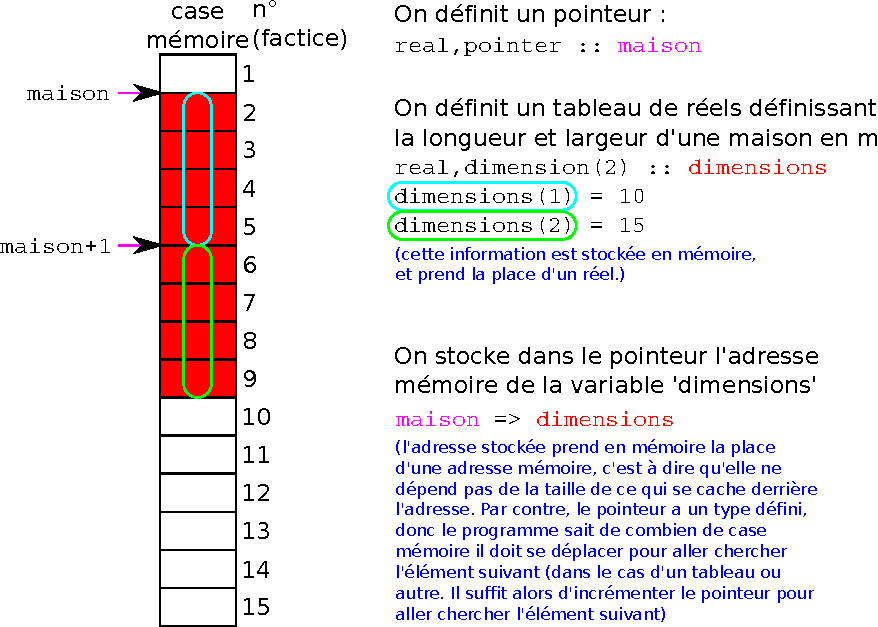
\includegraphics[width=0.65\linewidth]{figure/pointeurs.pdf}
\caption{Représentation schématique du fonctionnement d'un pointeur avec représentation de la mémoire. Les numéros pour les cases mémoires ne représentent pas la réalité, c'est juste pour montrer comment on fait référence à une case mémoire. L'idée est de montrer qu'en manipulant des adresses au lieu de manipuler les contenus, on peut faire des choses beaucoup plus puissantes.}
\end{figure}

On définit des pointeurs à l'aide d'attributs. Que ce soit pour définir les cibles que l'on pourra pointer
\begin{lstlisting}[language=Fortran]
real, target :: a, b(1000), c(10,10)
\end{lstlisting}
ou pour définir les pointeurs eux mêmes (qui devront bien évidemment avoir le même type que les cibles auxquelles ils seront associés ultérieurement)
\begin{lstlisting}[language=Fortran]
real, pointer :: pa, pb, pc
\end{lstlisting}

Pour attribuer une adresse au pointeur, il suffit ensuite de faire
\begin{verbatim}
pa => a
\end{verbatim}

Après cette assignation, on peut alors faire 
\begin{verbatim}
b(i) = pa * c(i,i)
\end{verbatim}
qui est équivalent en terme de résultat avec
\begin{verbatim}
b(i) = a * c(i,i)
\end{verbatim}

\bigskip

On peut aussi faire 
\begin{verbatim}
pa = 1.23456
write(*,*) 'a = ',a
\end{verbatim}
et avoir ``1.23456'' comme résultat affiché parce que changer \textit{pa} change \textit{a}

\bigskip

Le pointeur peut être ré-associé à n'importe quel moment. Il peut aussi être forcé à ne pointer sur rien en faisant : 
\begin{verbatim}
nullify(pa)
\end{verbatim}

\subsection{Attributs des variables lors de leur déclaration}
Lors de leur déclaration, il existe divers attributs que l'on peut donner aux variables et qui permettent de préciser à quoi elles vont servir notamment. 

\subsubsection{Une constante : parameter}

On peut ainsi définir une variable comme étant un paramètre, c'est à dire que cette dernière ne pourra pas être modifiée dans le reste du programme. C'est pratique pour définir des constantes comme la valeur de $\pi$ par exemple : 
\begin{lstlisting}[language=Fortran]
real, parameter :: pi = 3.14159
\end{lstlisting}

\subsubsection{Entrée ou sortie : intent}

Il est possible en Fortran 90 d'associer des attributs aux arguments des procédures pour fiabiliser les programmes. Les principaux attributs sont : 
\begin{itemize}
\item  \texttt{intent(in)}. Cet attribut signifie que la variable à laquelle il se rapporte est un argument d'entrée de la procédure ; sa valeur ne peut pas être modifiée par la procédure. 

\item  \texttt{intent(out)}. L'argument de la procédure a l'attribut sortie ; la procédure ne peut pas utiliser sa valeur. Elle doit en revanche lui en attribuer une.

\item  \texttt{intent(in/out)}. L'argument correspondant est à la fois un argument d'entrée (la procédure peut utiliser sa valeur) et un argument de sortie (la procédure doit lui en attribuer une nouvelle). 
\end{itemize}
Si les conditions précédentes ne sont pas respectées, une erreur surviendra à la compilation. La syntaxe des attributs est la suivante~: 
\begin{lstlisting}[language=Fortran]
subroutine nom(a, b, c)
 
implicit none         
integer, intent(in) ::   a       ! argument d'entree 
real, intent(out) ::   b         ! argument de sortie 
logical, intent(inout) ::   c    ! argument d'entree et de sortie
 
[...]         ! bloc d'instructions
 
end subroutine nom 
\end{lstlisting}

\subsection{Débuger des programmes fortran avec gdb}\index{gdb}\index{débugeur}
Afin d'utiliser un débugeur comme \gras{gdb} pour suivre l'exécution d'un programme fortran, il est nécessaire de le compiler avec l'option \texttt{-g}, par exemple : 
\begin{verbatim}
f77 -g foo.f -o foo
\end{verbatim}
La commande suivante va créer un exécutable \textbf{foo} que vous pouvez exécuter normalement ou à travers \textbf{gdb} pour suivre ce qu'il fait au fur et à mesure.

\bigskip

Pour commencer l'exécution du programme \textbf{foo} avec \textbf{gdb} il faut : 
\begin{enumerate}
\item faire précéder le nom du programme par \textbf{gdb} : 
\begin{verbatim}
gdb foo
\end{verbatim}
Vous aurez alors une ligne de commande de la forme 
\begin{verbatim}
(gdb) 
\end{verbatim}
\item entrez ces commandes dans le prompt \texttt{(gdb)} :
\begin{verbatim}
break main
run
\end{verbatim}
Ceci lancera l'exécution du programme, puis cette dernière sera mise en pause juste avant la première commande exécutable.
\end{enumerate}

\bigskip

Une chose intéressante à connaître est la séquence exacte d'exécution du programme, en particulier à travers les boucles et les tests conditionnels. Si le programme n'est pas trop gros, vous pouvez suivre facilement ce chemin en exécutant les lignes de code une à une. 

Pour exécuter la ligne suivante, il faut entrer dans le prompt \texttt{(gdb)} :
\begin{verbatim}
step
\end{verbatim}

À chaque fois que vous entrez la commande \texttt{step}, \textbf{gdb} va alors afficher la ligne qui est sur le point d'être exécuter, avec le numéro de ligne à gauche. Ceci permet de savoir ce qu'il va se passer, avant que ça ne se passe réellement.

\bigskip

Pour quitter \textbf{gdb}, entrez la commande suivante dans le prompt : 
\begin{verbatim}
quit
\end{verbatim}
Vous aurez alors le message suivant : 
\begin{verbatim}
The program is running.  Quit anyway (and kill it)? (y or n)
\end{verbatim}
Entrez '\texttt{y}' pour confirmez que vous souhaitez quitter \textbf{gdb}.

\subsubsection{Débuguer à l'aide d'un core dumped}
Parfois, il arrive qu'un programme plante et laisse un message du style
\begin{verbatim}
line 3: 37036 Abandon                 (core dumped) /home/login/bin/mercury/mercury
\end{verbatim}

Il est possible de lire ce fichier \textbf{core.37036} (dans mon cas) à l'aide de \textbf{gdb} en lançant une commande de ce style :
\begin{verbatim}
gdb /home/login/bin/mercury/mercury -c core.37036 
\end{verbatim}
où \textbf{/home/login/bin/mercury/mercury} est le chemin absolu vers le binaire concerné, ici \textbf{mercury}.

Vous devriez obtenir des informations du style :
\begin{verbatim}
GNU gdb (GDB) Fedora (7.2-26.fc14)
[.
.
.]
Core was generated by `/home/cossou/bin/mercury/mercury'.
Program terminated with signal 6, Aborted.
#0  0x00000038fdc34085 in raise () from /lib64/libc.so.6
Missing separate debuginfos, use: debuginfo-install glibc-2.12.90-21.x86_64 
libgcc-4.5.1-4.fc14.x86_64 libgfortran-4.5.1-4.fc14.x86_64
\end{verbatim}

En entrant la commande \textbf{where} vous aurez, avec un peu de chance, des informations sur l'endroit du plantage :
\begin{verbatim}
(gdb) where
#0  0x00000038fdc34085 in raise () from /lib64/libc.so.6
#1  0x00000038fdc35a36 in abort () from /lib64/libc.so.6
#2  0x00000038fdc7156b in __libc_message () from /lib64/libc.so.6
#3  0x00000038fdc76e26 in malloc_printerr () from /lib64/libc.so.6
#4  0x0000000000424aa6 in __algo_hybrid_MOD_mdt_hy ()
#5  0x0000000000404810 in mal_hcon.1587.clone.3 ()
#6  0x000000000040db8d in MAIN__ ()
#7  0x000000000040f43f in main ()
\end{verbatim}

Mais ces informations ne sont pas suffisantes. Pour avoir plus d'information, il suffit de recompiler votre programme avec l'option \textbf{-g} (pour \textbf{gfortran}), option pour donner plus d'information à \textbf{gdb}. Pas besoin de réexécuter la simulation. J'ai pour ma part compilé à coté, et je n'ai même pas quitté \textbf{gdb} pendant le processus. 

Puis, il faut charger le fichier binaire compilé avec l'option pour \textbf{gdb} en faisant dans gdb :
\begin{verbatim}
(gdb) file /home/cossou/bin/mercury/mercury
warning: exec file is newer than core file.
Reading symbols from /home/cossou/bin/mercury/mercury...done.
\end{verbatim}
J'ai eu droit à ce warning, c'est normal, vu que je viens de le compiler. Mais je n'ai rien changé par ailleurs. Et un nouveau \textbf{where} me donne les informations suivante :
\begin{verbatim}
(gdb) where
#0  0x00000038fdc34085 in raise () from /lib64/libc.so.6
#1  0x00000038fdc35a36 in abort () from /lib64/libc.so.6
#2  0x00000038fdc7156b in __libc_message () from /lib64/libc.so.6
#3  0x00000038fdc76e26 in malloc_printerr () from /lib64/libc.so.6
#4  0x0000000000424aa6 in algo_hybrid::mdt_hy (time=313506736, h0=8, 
    tol=9.9999999999999998e-13, en=..., am=<value optimized out>, jcen=..., 
    rcen=0.0050000000000000001, nbod=30, nbig=30, m=..., x=..., v=..., s=..., 
    rphys=..., rcrit=..., rce=..., stat=..., id=..., ngf=..., dtflag=2, 
    ngflag=0, opflag=0, colflag=0, nclo=0, iclo=..., jclo=..., dclo=..., 
    tclo=..., ixvclo=..., jxvclo=..., _id=8) at algo_hybrid.f90:96
#5  0x0000000000404810 in mal_hcon (time=313506736, h0=8, 
    tol=9.9999999999999998e-13, jcen=..., rcen=0.0050000000000000001, en=..., 
    am=..., cefac=3, ndump=500, nfun=100, nbod=30, nbig=30, m=..., xh=..., 
    vh=..., s=..., rho=..., rceh=..., stat=..., id=..., ngf=..., opflag=0, 
    ngflag=0, onestep=0x423e60 <algo_hybrid::mdt_hy>, 
    coord=0x422f20 <algo_hybrid::mco_h2dh>, 
    bcoord=0x422d20 <algo_hybrid::mco_dh2h>, _id=<value optimized out>)
    at mercury.f90:1256
#6  0x000000000040db8d in mercury () at mercury.f90:262
#7  0x000000000040f43f in main (argc=<value optimized out>, 
    argv=<value optimized out>) at mercury.f90:114
#8  0x00000038fdc1ee7d in __libc_start_main () from /lib64/libc.so.6
#9  0x00000000004010e9 in _start ()
\end{verbatim}

\begin{important}
Le point crucial est que dans mon cas, je peux récupérer le temps précis du plantage, et ainsi relancer la simulation (je peux repartir d'un fichier dump juste avant le crash, donc quasi immédiat), mais exécuter avec une version modifiée de mercury qui me donne plein d'informations sur la simulation uniquement quand le temps est égal au temps du crash et un petit peu avant.)

Le temps est ici un paramètre de la routine \verb|mdt_hy (time=313506736 ...)| ce qui me permet de rajouter le bout de code suivant dans mon programme : 
\begin{verbatim}
if (time.gt.313506725) then
  open(10, file='leak.out', status="old", access="append")
  write(10,*) time, planet, time_mig, time_ecc, time_inc
  close(10)
  write(*,*)
  call print_planet_properties(p_prop)
end if
\end{verbatim}
\end{important}

\subsubsection{Savoir où on se trouve dans le programme}
Pour savoir où on est, il suffit d'entrer dans le prompt \texttt{(gdb)} :
\begin{verbatim}
where
\end{verbatim}
Cette commande affiche alors le numéro de ligne de la ligne courante. par exemple quelque chose du genre : 
\begin{verbatim}
#0  foo () at foo.f:12
\end{verbatim}
indique que l'exécution du programme est actuellement au niveau de la ligne 12 du code source du fichier \textbf{foo.f}

\bigskip

Vous pouvez afficher quelques lignes du code source autour de la position actuelle via 
\begin{verbatim}
list
\end{verbatim}

Il est aussi possible, via cette commande, de spécifier une liste de lignes à afficher. Par exemple pour lister les lignes 10 à 24 du programme courant, vous devez entrer dans le prompt \texttt{(gdb)} :
\begin{verbatim}
list 10,24
\end{verbatim}

\subsubsection{Afficher le contenu d'une variable fortran avec gdb}
À n'importe quel moment de l'exécution pas à pas du programme, vous pouvez connaître les valeurs courantes de vos variables en utilisant la commande \texttt{print}. Par exemple, si vous avez une variable \textbf{density}, vous pouvez entrer la commande suivante afin de connaître la valeur stockée : 
\begin{verbatim}
print density
\end{verbatim}
 
\begin{attention}
Vous devez entrer les noms des variables en minuscules dans \textbf{gdb}, sans vous préoccuper de la casse de la variable dans votre code source.
\end{attention}

\subsubsection{Mettre le programme en pause à un endroit particulier}
Au lieu d'entrer 
\begin{verbatim}
break main
\end{verbatim}
il faut entrer une commande du style
\begin{verbatim}
break [file:]function
\end{verbatim}
où \texttt{[file:]} est un argument optionnel qui permet de spécifier dans quel fichier se trouve la fonction considérée (s'il y a plusieurs fichiers) et \texttt{function} est le nom de la fonction au début de laquelle on veut mettre l'exécution en pause.

\subsubsection{Débuggage avancé}
Pour exécuter le programme ligne à ligne, il existe \texttt{next} et \texttt{step}. 
\begin{enumerate}
\item \texttt{step} permet d'exécuter la ligne suivante du programme tout en passant \emph{au-dessus} de tout appel de fonction dans la ligne.
\item \texttt{next} permet d'exécuter la ligne suivante du programme, en exécutant aussi tous les appels de fonctions de la ligne.
\end{enumerate}


\bigskip

Pour continuer l'exécution (jusqu'au prochain breakpoint je suppose) il faut utiliser la commande suivante dans le prompt \textbf{(gdb)} :
\begin{verbatim}
c
\end{verbatim}

\begin{remarque}
En compilant avec \textbf{gfortran} et l'option \texttt{-fbounds-check}, il faut lancer l'exécutable et les tests seront effectués au cours de l'exécution si j'ai bien compris, même si des tests sont effectués au cours de la compilation aussi.
\end{remarque}


\subsection{Erreurs de compilation}
\subsubsection{Utilisation de fonctions internes à un module}
\begin{verbatim}
kepler_equation.o: In function `__kepler_equation_MOD_orbel_fhybrid':
kepler_equation.f90:(.text+0x25f): undefined reference to `orbel_flon_'
collect2: ld a retourné 1 code d'état d'exécution
\end{verbatim}

Le problème vient de la fonction \verb|orbel_fhybrid| du module \verb|kepler_equation|. j'ai en effet pris des fonctions pour en faire un module, et avant, des variables étaient définies dans la fonction, puisque celle-ci faisait appel à d'autres fonctions. Toutes ces fonctions faisant maintenant partie du même module, on peut et on doit enlever ces définitions. 

Pour résoudre le problème, j'ai donc supprimé la ligne : 
\begin{verbatim}
real*8 orbel_flon
\end{verbatim}
dans la définition de la fonction \verb|orbel_fhybrid|.

\subsubsection{Utilisation de fonctions d'un module}
\begin{verbatim}
mercury.f90:1140.22:

  character*8 mio_re2c, mio_fl2c
                      1
Error: Symbol 'mio_re2c' at (1) already has basic type of CHARACTER
\end{verbatim}
Il faut supprimer cette ligne parce que le type de la fonction est déjà défini dans le module, pas besoin de redéfinir le type de la fonction dans la subroutine qui importe le module.

\subsubsection{Utilisation de subroutine en paramètre d'autres subroutines}
\begin{verbatim}
mercury.f90:137.19:

  external mco_dh2h,mco_h2dh
                   1
Error: Cannot change attributes of USE-associated symbol at (1)
\end{verbatim}

En mettant ces subroutines (celles qu'on appelle en argument) dans un module, pas besoin de les définir via un \texttt{external}. Il faut donc supprimer cette ligne.

\subsubsection{Function has no implicit type}
\begin{verbatim}
test_mfo_user.f90:35.12:

      f_p = get_F(p)
            1
Error: Function 'get_f' at (1) has no IMPLICIT type
\end{verbatim}

J'ai eu cette erreur parce que je n'avais pas rajouté le module dans la ligne de compilation 
\begin{verbatim}
gfortran -o test test_mfo_user.f90 user_module.o
\end{verbatim}

\bigskip

J'ai eu aussi cette erreur parce que dans le module \textbf{user\_module}, la fonction \textbf{get\_F} était une fonction privée.

\subsubsection{Error: Rank mismatch in array reference at (1) (2/1)}
J'avais cette erreur parce que j'avais déclaré la variable comme 
\begin{lstlisting}[{language=fortran}]
real, dimension(:), intent(in) :: matrix
\end{lstlisting}
au lieu de
\begin{lstlisting}[{language=fortran}]
real, dimension(:,:), intent(in) :: matrix
\end{lstlisting}
Il lui manquait donc une dimension. Et ça buguait quand je voulais faire :
\begin{lstlisting}[{language=fortran}]
temp = matrix(i,j) + 1.
\end{lstlisting}

\subsubsection{Error: Rank mismatch in argument 'levels' at (1) (1 and 0)}
Dans la routine, j'avais
\begin{lstlisting}[{language=fortran}]
real, dimension(:), intent(in) :: levels
\end{lstlisting}
et j'essayais de passer en argument
\begin{lstlisting}[{language=fortran}]
call contour(levels=0.)
\end{lstlisting}
Le problème vient du fait qu'on ne peut pas passer un scalaire pour un argument défini comme étant un tableau, il ne comprend pas que ça peut être un tableau à un élément. Je n'ai pas vraiment résolu le problème puisque je l'ai contourné en définissant l'argument comme scalaire. Je ne sais pas comment faire pour qu'on puisse passer une seule valeur. Peut-être définir un tableau à un seul élément via \texttt{dimension(1)}.
\end{document}